\documentclass[11pt]{article}

\usepackage[a4paper,margin=1in]{geometry}
\usepackage[T1]{fontenc}
\usepackage[utf8]{inputenc}
\usepackage{lmodern}
\usepackage{graphicx}
\usepackage{subcaption}
\usepackage{booktabs}
\usepackage{hyperref}
\usepackage{float}
\usepackage{tabularx}
\usepackage{longtable}
\usepackage{array}
\usepackage{makecell}
\usepackage{ragged2e}
\usepackage{adjustbox}
\usepackage{xurl}
\usepackage{seqsplit}
\usepackage{microtype}
\usepackage{setspace}
\usepackage{amsmath}
\usepackage{tikz}
\usetikzlibrary{arrows.meta, positioning, fit, calc, shapes.geometric}

\newcolumntype{L}[1]{>{\RaggedRight\arraybackslash}p{#1}}
\newcolumntype{Y}{>{\RaggedRight\arraybackslash}X}
\newcommand{\code}[1]{\path{#1}}
\newcommand{\pathcode}[1]{\path{#1}}

\title{City1: A Reproducible Calibrated and Uncertainty-Aware Proxy Population Surface Framework for Intra-Urban Analysis in Data-Scarce Kazakhstan}
\author{}
\date{}

\begin{document}

\maketitle

\begin{abstract}
In Kazakhstan and similar data-scarce urban settings, official city totals may be available while true cell-level census labels are not. This creates a two-part methodological problem: first, how to construct a reproducible calibrated proxy population surface under missing cell-level truth; second, how to prevent that deterministic surface from being over-read as equally reliable everywhere. City1 addresses both stages within one framework. Stage 1 builds a fixed 500 m calibrated proxy population surface from OpenStreetMap-derived features, weak target construction, Random Forest modeling, and official-total calibration. Stage 2 adds a reliability-aware interpretation layer through calibrated ensemble predictions, P10/P50/P90 proxy intervals, uncertainty width, relative uncertainty, confidence bands, and hotspot prioritization classes. The baseline stage is supported by leave-one-city-out transfer testing, spatial block cross-validation, grid benchmarking, OSM completeness assessment, district aggregation evidence, external structural comparison, ablation, and qualitative plausibility review. The uncertainty-aware stage is supported most strongly by hotspot stability and confidence-band separation of uncertainty burden; interval coverage is mixed, external disagreement alignment is mixed or negative, and district interval coverage remains partial. The framework therefore does not reconstruct true cell-level census counts and does not estimate true census uncertainty. Instead, it contributes a transparent, reproducible, officially calibrated, and uncertainty-aware proxy population framework for screening and interpretation under missing cell-level truth.

\end{abstract}

\section{Introduction}

Spatially explicit intra-urban population surfaces are useful for service planning, hotspot screening, exposure assessment, urban comparison, and first-pass neighborhood analysis. Many practical decisions depend not only on total city population but also on how population is distributed across the urban fabric. Yet in data-scarce settings, the population is usually observed only through aggregated administrative counts rather than through true cell-level census labels \cite{Leyk2019,Mennis2009,Stevens2015}. This creates an immediate methodological asymmetry: the spatial product that urban analysis needs is finer than the population data that are actually observed.

In Kazakhstan and similar contexts, this asymmetry is especially important. Official city totals may exist and can be verified, but fine-resolution cell-level truth is unavailable for direct supervised learning. At the same time, open geospatial data such as buildings, roads, and points of interest provide a reproducible but indirect description of the urban environment. These signals do not reveal the true population count in each cell, but they can support a bounded proxy modeling workflow when linked to official totals and explicit allocation logic.

This problem has two linked parts. First, a reproducible calibrated proxy population surface must be constructed and validated under missing cell-level truth. Second, once that surface exists, users still need to know where it appears more stable and where it should be treated more cautiously. A deterministic surface that assigns one value per cell can otherwise encourage over-reading by making all cells look equally trustworthy. The scientific need is therefore not only for a calibrated proxy surface, but for a reliability-aware interpretation layer around that surface. Put differently, Stage 1 answers whether a bounded proxy surface can be built at all, while Stage 2 answers how that surface should be read once it exists.

City1 addresses these two research questions as one framework paper:

\begin{itemize}
\item \textbf{RQ1:} How can a reproducible calibrated proxy population surface be constructed under missing cell-level census truth?
\item \textbf{RQ2:} Once such a proxy surface is constructed, how can uncertainty, confidence, and hotspot stability be represented so that users do not over-read deterministic cell-level patterns?
\end{itemize}

The framework follows one mandatory transition logic. First, it constructs and validates a deterministic calibrated proxy surface under missing cell-level truth. Second, it extends this surface with uncertainty-aware interpretation, so that the output is not only spatially explicit but also reliability-aware.

\paragraph{Unified contributions.}
\begin{itemize}
\item a reproducible open-data proxy population surface pipeline based on weak supervision, Random Forest modeling, a fixed 500 m grid, and official-total calibration;
\item a multi-level validation stack for structural credibility under missing cell-level truth;
\item an uncertainty-aware extension built from calibrated ensemble intervals, relative uncertainty, and bounded confidence bands;
\item confidence-aware hotspot prioritization that separates stronger screening candidates from review-oriented ones;
\item an integrated evidence package in which figures, tables, formulas, limitations, and supplement material remain traceable to reference artifacts rather than to moving experimental targets.
\end{itemize}

Table~\ref{tab:contribution-map} summarizes these contributions as one two-stage framework rather than as two pasted papers. It is the roadmap for the paper, not a decorative summary.

\begin{table}[H]
\centering
\scriptsize
\caption{Contribution Map for the unified City1 framework. The table makes explicit how the calibrated baseline stage and the uncertainty-aware stage connect within one paper.}
\label{tab:contribution-map}
\begin{tabular}{p{3.0cm}p{1.2cm}p{3.0cm}p{3.0cm}p{3.8cm}}
\toprule
Contribution & Stage & Method / artifact & Main evidence & Claim boundary \\
\midrule
Reproducible calibrated proxy population surface & Stage 1 & weak target, Random Forest, 500 m grid, official-total calibration & LOCO, spatial block CV, grid benchmark, external benchmark, ablation & supports proxy-surface credibility, not cell-level census truth \\
Multi-level structural validation & Stage 1 & district benchmark, WorldPop/GHS-POP comparison, qualitative plausibility & district, external, and qualitative evidence & supports structural plausibility, not ground-truth validation \\
Uncertainty-aware interpretation layer & Stage 2 & calibrated ensemble, P10/P50/P90, interval width, relative uncertainty & interval coverage and error-width alignment & supports bounded uncertainty behavior, not true census uncertainty \\
Confidence-aware hotspot prioritization & Stage 2 & confidence bands and hotspot classes & confidence-band separation and hotspot stability & supports screening reliability, not verified population-hotspot truth \\
Tool-grounded interpretation layer & Stage 3 & read-only evidence tools, deterministic fallback, optional provider generation, cache support, and guardrails & bounded evaluation of evidence-linked explanation and safety behavior & supports reviewer-safe interpretation, not new population estimation or automated policy evidence \\
\bottomrule
\end{tabular}
\end{table}


The scientific identity of the paper is intentionally bounded. City1 does not reconstruct true cell-level census counts. It does not estimate true census uncertainty. Instead, it produces an officially calibrated proxy population surface and then adds a reliability-aware interpretation layer so that the resulting surface can be used more responsibly for screening and exploratory urban analysis. Within those bounds, the contribution is not merely a map. The contribution is a disciplined framework for producing, validating, and interpreting a calibrated proxy population surface under missing cell-level truth.

The rest of the manuscript follows this roadmap in order: Stage 1 constructs and validates the calibrated proxy baseline, Stage 2 explains how to interpret that baseline cautiously, and the discussion then connects the two stages into one coherent framework.

\section{Related Work}

\subsection{Gridded population mapping and dasymetric redistribution}

Gridded population mapping has evolved from simple areal representations toward increasingly sophisticated methods for redistributing aggregated totals into regular grid cells \cite{Leyk2019,Mennis2009}. A major branch of this literature uses top-down redistribution: official or census-based counts are allocated across space with land cover, built-up area, buildings, infrastructure, or other ancillary covariates \cite{Mennis2009,Stevens2015}. This logic is closely related to dasymetric mapping, where ancillary spatial evidence constrains where population can plausibly be allocated within a larger reporting unit.

Large-scale products such as WorldPop and the Global Human Settlement Layer are especially relevant here because they show both the usefulness and the limits of gridded population products. WorldPop combines administrative counts with geospatial covariates in model-based redistribution workflows, including random-forest-based disaggregation \cite{Stevens2015,Sorichetta2015,Lloyd2017,WorldPopMethods}. GHS-POP and related GHSL tools emphasize transparent built-up-anchored redistribution frameworks at global scale \cite{Freire2016,GHSL2023,GHSPOP2G2020}. Both families are scientifically useful comparators, but neither should be mistaken for cell-level ground truth in every city.

\subsection{Proxy modeling under missing cell-level truth}

In local urban settings, the central challenge is often not the absence of population information altogether, but the mismatch between the coarse level at which population is observed and the fine level at which analysts want to work. Recent studies therefore use combinations of buildings, roads, points of interest, and other geospatial features to derive proxy or model-based population surfaces \cite{Qiu2020,Pirowski2024,Popcorn2024}. In these settings, official totals can still anchor the city-level mass even when cell-level truth is unavailable.

This is where weak targets become methodologically important. Rather than pretending that a hidden census can be directly observed, weak-target workflows construct a structured proxy target from available spatial signals and then learn against that bounded target. The resulting product is best understood as a calibrated proxy surface rather than a true cell-level census surface.

\subsection{Need for uncertainty-aware interpretation}

Validation under missing cell-level truth is intrinsically multi-layered. Weak targets, aggregated administrative checks, external structural comparison, and qualitative plausibility can each contribute evidence, but none of them alone resolves cell-level truth \cite{Leyk2019,Thomson2021,Yin2021}. This creates an additional interpretive problem: a deterministic proxy surface can look uniformly authoritative even when support conditions vary materially across cities and within cities.

That gap motivates the uncertainty-aware stage of City1. The objective is not to convert a proxy surface into a true census-uncertainty model. The objective is to show where the calibrated proxy surface appears more stable, where it appears weaker, and where hotspot screening should be treated more cautiously. In this sense, the uncertainty-aware extension is a reliability-aware interpretation layer built on top of the calibrated baseline, not a replacement of the baseline task identity.

This also aligns the paper with a broader fitness-for-use perspective: the question is not only whether a proxy surface can be produced, but whether it can be read responsibly for the task at hand. City1 answers that question by pairing calibration with a bounded interpretation layer.

\section{Study Design and Data}

The study focuses on Kazakhstan as a data-scarce urban setting in which official city totals are available but true grid-level population labels are not. This makes the national setting methodologically central rather than incidental. The framework is designed for a context where city-level accounting can be anchored to verified totals, while intra-urban structure must be inferred from open geospatial evidence under explicit uncertainty and limitation boundaries.

The broader deterministic baseline is organized around a 10-city reference registry with official totals available for calibrated inference: Almaty, Astana, Shymkent, Semey, Kurchatov, Taraz, Uralsk, Petropavlovsk, Ust Kamenogorsk, and Ridder. Within that registry, 8 cities form the validated baseline batch with the full combination of official totals, feature generation, and baseline evidence support: Almaty, Astana, Shymkent, Semey, Kurchatov, Taraz, Uralsk, and Petropavlovsk. Kurchatov and Ridder remain important for calibrated runtime support or official-total registry coverage, even though they do not carry the full deeper validation stack. Semey is additionally retained as a smoke-passed example city in the reference package. This is not an inconsistency. It is a layered evidence design in which the registry, the baseline validation batch, and the uncertainty-evidence subset answer different scientific questions at different depths.

Official city totals act as calibration anchors throughout the framework. The canonical reference is \texttt{data/external/city\_population\_reference\_v2.csv}, with supported totals fixed to the reference date 2026-02-01. In the reference package, Almaty, Astana, and Shymkent are tied to Bureau of National Statistics regional statistics page values, while the other supported cities are compiled through cached BNS regional monthly workbooks. The companion registry \texttt{data/external/city\_status\_registry\_v2.csv} records which cities belong to the validated baseline, the smoke-tested examples, and the broader support frame.

The feature layer is derived from OpenStreetMap and grouped into built form, floor-area proxies, transport structure, and point-of-interest or service-access variables. This design reflects the bounded premise of the framework: in the absence of true cell-level census labels, the target is not truth reconstruction but a transparent calibrated proxy surface supported by reproducible open-data inputs. The production grid is fixed to 500 m for both analytical stages.

The study design also distinguishes between the broader baseline registry and the narrower reliability-evidence subset. District benchmark comparison is available for Almaty, Astana, and Shymkent. Qualitative plausibility review is locked to Almaty and Astana as two deliberately contrasting visual reading contexts. External structural comparison is conducted against WorldPop and GHS-POP. OSM completeness is retained as input-support context rather than as a performance label.

The uncertainty-aware extension then focuses on a four-city inference package: Almaty, Astana, Semey, and Shymkent. This subset is used to test reliability-aware interpretation, confidence-band separation, interval behavior, and hotspot screening. It does not replace the broader deterministic 10-city reference frame. Instead, the relationship is explicit: the deterministic baseline uses the broader registry and validation stack, whereas the uncertainty-aware extension uses the four-city package to assess where the calibrated proxy surface is stronger, weaker, or caution-heavier.

Seen together, the study design therefore behaves like a staged evidence ladder. The widest registry supports reproducibility and coverage. The eight-city baseline supports the main deterministic claims. The three district benchmark cities and two qualitative plausibility cities support specific kinds of credibility checks. The four-city uncertainty package supports reliability-aware interpretation. Each subset is narrower for a reason, and each reason is traceable to the claim boundary it is supposed to support.

\input{tables_tex/table2_study_coverage_summary.tex}

\section{Deterministic Calibrated Proxy Surface Method}

\subsection{Spatial grid and feature extraction}

The first stage of City1 constructs a deterministic calibrated proxy population surface on a fixed 500 m grid. Each city is partitioned into regular grid cells, and all downstream feature aggregation, weak-target construction, learning, calibration, and validation are carried out at that spatial unit.

Input features are derived from OpenStreetMap and grouped into interpretable urban proxy families. Built-form and floor-area variables provide proxies for horizontal and vertical development intensity, transport variables provide a coarse proxy for corridor structure and accessibility, and service or point-of-interest variables provide activity and amenity concentration context. These variables are not treated as direct census truth. They form the transparent open-data evidence layer on which the calibrated proxy surface is built.

\subsection{Weak target construction}

Because true cell-level census labels are unavailable, the deterministic stage uses weak supervision. Rather than training directly on observed population counts per cell, it first builds a proxy score intended to reflect relative intra-urban population concentration.

Let $x_{ik}$ denote feature $k$ for cell $i$, and let $K$ denote the subset of weak-label features available in city $c$. In the reference workflow, negative values are clipped, features are log-transformed, and then min-max normalized before fixed weak-label weights are applied:
\[
s_i = \sum_{k \in K} w_k \cdot \mathrm{MinMax}\!\left(\log\!\left(1 + \max(x_{ik}, 0)\right)\right).
\]

To avoid zero-share collapse at allocation time, the proxy score is shifted by a small constant $\epsilon$ and converted into a city-wise allocation share:
\[
\tilde{s}_i = s_i + \epsilon,
\qquad
q_i = \frac{\tilde{s}_i}{\sum_{j \in c} \tilde{s}_j},
\qquad
y_i^{\mathrm{weak}} = q_i \cdot P_c,
\]
where $P_c$ is the official city total for city $c$. The resulting weak target is therefore an officially anchored proxy allocation, not an observed cell-level census label.

This construction is intentionally circular in a limited sense, because the target inherits structure from the same proxy evidence that later enters the model. That circularity is acceptable only because the paper does not present the target as truth. Instead, the target is a transparent allocation device that tells the learning system how to distribute city mass across cells under a bounded proxy framework. In other words, the model is being asked to learn a calibrated proxy allocation pattern, not to rediscover hidden census truth.

\subsection{Supervised learning on weak targets}

The deterministic stage then learns a mapping from the OSM-derived feature space to the weak target surface. The main production model is Random Forest, while ridge regression is retained as a deliberately simple linear comparator within the same target and calibration regime. The purpose of the learning stage is not to recover hidden truth directly, but to learn a stable and transferable relationship between open-data urban structure and the weakly supervised proxy distribution.

The model is trained on a calibrated proxy target, not on true cell-level census observations. This distinction is central to the framework and remains explicit throughout the manuscript. Validation against weak targets therefore supports proxy-surface credibility, not true population accuracy. The gain is methodological transparency: the framework tells the reader exactly which evidence was used to allocate city totals, and exactly how far that evidence can be trusted.

\subsection{Random Forest production model and ridge comparator}

The fixed production identity of the deterministic stage is Random Forest on the 500 m grid in calibrated-only mode. Ridge regression is retained as a baseline comparator because it provides a transparent contrast between a flexible non-linear model and a simple standardized linear model. In the reference workflow, ridge uses the same feature columns, the same weak target, the same log-target transform, and the same official-total calibration logic as Random Forest. The comparison therefore remains traceable to one coherent baseline stack rather than to unrelated model families.

Ridge is not used as an exhaustive search over all possible linear alternatives. It is retained as a simple comparator that helps show why a non-linear learner is justified for urban proxy allocation. The point is not that ridge fails in a vacuum, but that the final production identity is more credible when the manuscript shows a transparent linear benchmark and then justifies why Random Forest is the stronger fixed configuration.

\subsection{Calibration to official city totals}

Raw model predictions are treated as relative cell-level outputs before final city-total anchoring. The deterministic surface is then calibrated so that the sum of all cells within a city matches the corresponding official total:
\[
\hat{y}_i^{\mathrm{cal}} = \hat{y}_i \cdot \frac{P_c}{\sum_{j \in c}\hat{y}_j}.
\]
If the within-city prediction sum is non-positive, the workflow falls back to a uniform allocation across the cells of that city so that calibration remains well defined even under degenerate raw output.

Calibration guarantees city-level consistency, but it does not convert the output into cell-level census truth. The calibrated surface should therefore be interpreted as an officially constrained proxy population surface whose value lies in transparency, reproducibility, and bounded structural credibility.

The calibration step is not a cosmetic post-processing detail. It is part of the scientific construction of the final product because it anchors the city-wide mass that the weak target was designed to distribute. The final output is therefore a learned allocation constrained by official totals, not an unconstrained prediction surface.

\subsection{Fixed production identity}

The deterministic stage is intentionally locked to three choices: Random Forest, 500 m grid resolution, and calibrated-only output. This fixed identity matters because it prevents post hoc drift in claims and ensures that the reported tables, figures, and narrative conclusions all refer to one consistent production configuration. In the unified framework, this deterministic stage is the stable calibrated baseline that the uncertainty-aware extension later interprets rather than replaces.

\section{Uncertainty-Aware Extension}

Figure~\ref{fig:city1-framework} shows the full City1 framework. Stage 1 builds the deterministic calibrated proxy baseline. Stage 2 adds a reliability-aware interpretation layer so that the calibrated surface is not over-read as equally reliable everywhere. Stage 2 does not replace Stage 1. It consumes the calibrated baseline, asks how stable that baseline looks under ensemble variation, and then translates that stability into bounded screening categories.

\begin{figure}[H]
\centering
\resizebox{\textwidth}{!}{%
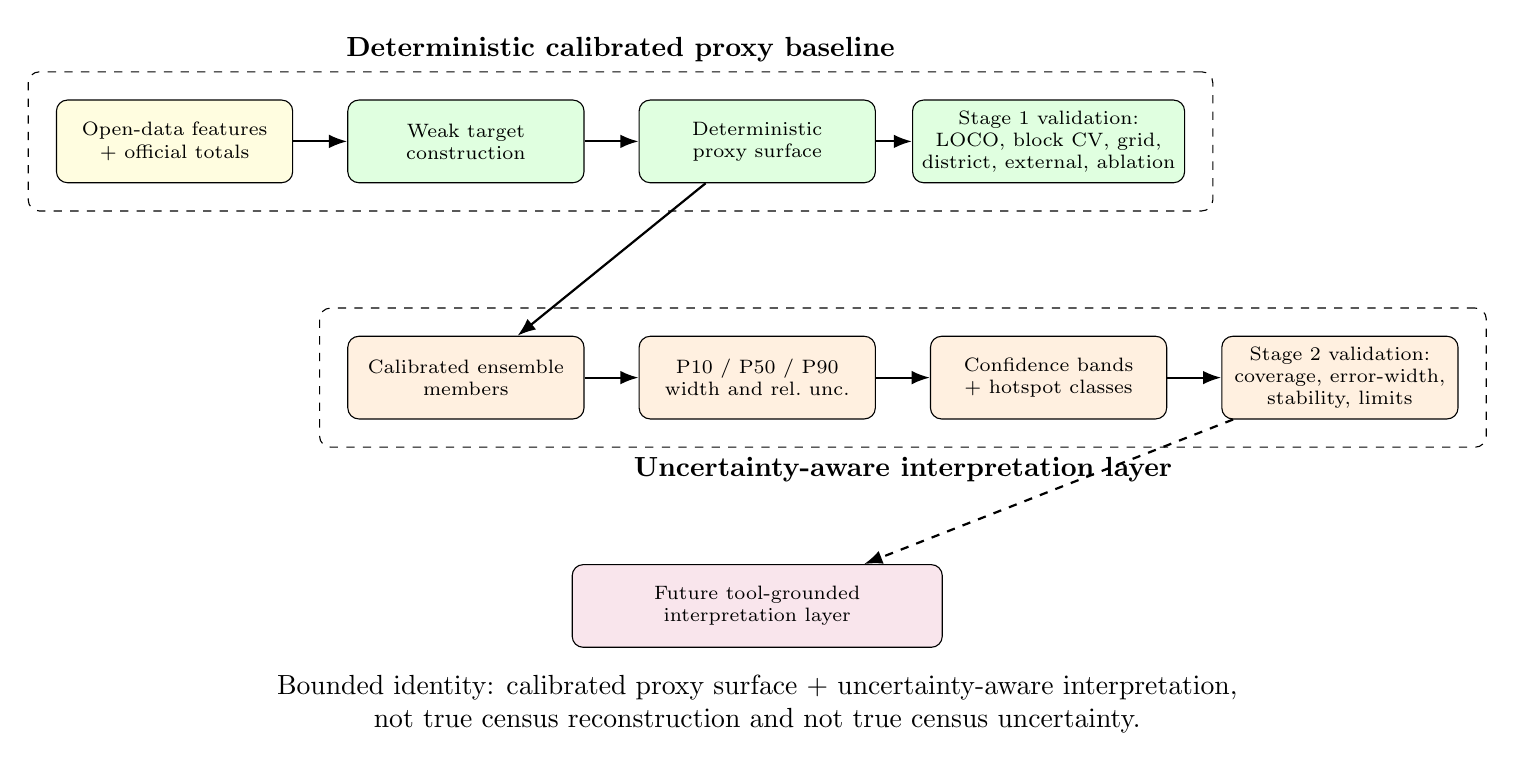
\begin{tikzpicture}[
  box/.style={draw, rounded corners, align=center, minimum width=3.0cm, minimum height=1.05cm, fill=blue!6, font=\scriptsize},
  stage/.style={draw, rounded corners, dashed, inner sep=10pt},
  arrow/.style={-Latex, thick}
]
\node[box, fill=yellow!12] (data) at (0,0) {Open-data features\\+ official totals};
\node[box, fill=green!12] (weak) at (3.7,0) {Weak target\\construction};
\node[box, fill=green!12] (det) at (7.4,0) {Deterministic\\proxy surface};
\node[box, fill=green!12] (val1) at (11.1,0) {Stage 1 validation:\\LOCO, block CV, grid,\\district, external, ablation};

\node[box, fill=orange!12] (ens) at (3.7,-3.0) {Calibrated ensemble\\members};
\node[box, fill=orange!12] (int) at (7.4,-3.0) {P10 / P50 / P90\\width and rel.\ unc.};
\node[box, fill=orange!12] (hot) at (11.1,-3.0) {Confidence bands\\+ hotspot classes};
\node[box, fill=orange!12] (val2) at (14.8,-3.0) {Stage 2 validation:\\coverage, error-width,\\stability, limits};

\node[box, fill=purple!10, minimum width=4.7cm] (future) at (7.4,-5.9) {Future tool-grounded\\interpretation layer};

\draw[arrow] (data) -- (weak);
\draw[arrow] (weak) -- (det);
\draw[arrow] (det) -- (val1);
\draw[arrow] (det) -- (ens);
\draw[arrow] (ens) -- (int);
\draw[arrow] (int) -- (hot);
\draw[arrow] (hot) -- (val2);
\draw[arrow, dashed] (val2) -- (future);

\node[stage, fit=(data)(weak)(det)(val1), label=above:{\textbf{Deterministic calibrated proxy baseline}}] {};
\node[stage, fit=(ens)(int)(hot)(val2), label=below:{\textbf{Uncertainty-aware interpretation layer}}] {};
\node[align=center] at (7.4,-7.15) {Bounded identity: calibrated proxy surface + uncertainty-aware interpretation,\\not true census reconstruction and not true census uncertainty.};
\end{tikzpicture}%
}

\caption{Unified City1 framework diagram. Stage 1 constructs and validates a deterministic calibrated proxy population surface under missing cell-level truth. Stage 2 extends that surface with calibrated ensemble intervals, confidence bands, and hotspot screening. Stage 3 then exposes the frozen evidence through a bounded tool-grounded interpretation and safety layer without altering the underlying population estimates.}
\label{fig:city1-framework}
\end{figure}

Stage 3 remains subordinate to the scientific artifacts produced earlier in the framework. It consumes frozen calibrated and uncertainty-aware outputs through controlled tools, deterministic fallback generation, optional provider generation, cache support, and claim-boundary guardrails. Its role is evidence-linked explanation and reviewer-safe interpretation, not new estimation, not truth recovery, and not automated policy decision-making.

\subsection{Ensemble Random Forest configuration}

The uncertainty-aware stage preserves the same fixed 500 m grid and the same 17 frozen feature columns used by the deterministic baseline, but wraps the production model in an ensemble-of-runs design. The reference uncertainty package uses 20 Random Forest members, within-city bootstrap resampling, log-target training, and a training package with 8 cities and 16,132 rows. The reference inference package covers four cities: Almaty, Astana, Semey, and Shymkent.

This is not a new truth model. It is an interpretation layer built on top of the calibrated proxy surface. The purpose is to expose reliability differences that are hidden if one only looks at the deterministic median surface.

\subsection{Calibrated ensemble members}

Let $\hat{y}^{(m)}_{i,c}$ denote the raw prediction for cell $i$ in city $c$ from ensemble member $m$. Each member is calibrated separately to the official city total $P_c$:
\[
\hat{y}^{(m),\mathrm{cal}}_{i,c}=
\hat{y}^{(m)}_{i,c}
\cdot
\frac{P_c}{\sum_{j \in c}\hat{y}^{(m)}_{j,c}},
\]
whenever the within-city raw sum is positive. If the raw sum is non-positive, the same uniform fallback logic is used as in the deterministic stage. This preserves the official-total accounting identity at the ensemble-member level rather than calibrating only after interval aggregation.

\subsection{P10/P50/P90 interval outputs}

The calibrated member ensemble is summarized per cell through empirical quantiles:
\[
\mathrm{P10}_i = Q_{0.10}\!\left(\hat{y}^{(m),\mathrm{cal}}_{i,c}\right), \qquad
\mathrm{P50}_i = Q_{0.50}\!\left(\hat{y}^{(m),\mathrm{cal}}_{i,c}\right), \qquad
\mathrm{P90}_i = Q_{0.90}\!\left(\hat{y}^{(m),\mathrm{cal}}_{i,c}\right).
\]
The median surface, $\mathrm{P50}$, is the canonical final proxy surface for the uncertainty-aware stage and remains the backward-compatible population estimate.

Interval width and relative uncertainty are defined as:
\[
\mathrm{width}_i = \mathrm{P90}_i - \mathrm{P10}_i,
\qquad
r_i = \frac{\mathrm{width}_i}{\max(\mathrm{P50}_i,\epsilon)}.
\]
These are proxy uncertainty summaries inside the calibrated proxy framework, not true census-uncertainty intervals.

The quantiles should therefore be read as a stability envelope around the proxy surface. P50 is the canonical surface for reporting, while P10 and P90 provide a bounded spread that helps distinguish cells with tighter support from cells with broader support. The point is not to claim probabilistic ground truth, but to prevent the median surface from being interpreted as equally certain everywhere.

\subsection{Confidence score and confidence bands}

The uncertainty-aware stage introduces a bounded interpretation-confidence score rather than a probability of correctness. A model-stability component first measures how large a cell's relative uncertainty is compared with the upper uncertainty tail in its city:
\[
s_i = 1 - \operatorname{clip}\!\left(
\frac{r_i}{\max(q_{0.90}^{(c)},\epsilon)}, 0, 1
\right).
\]
This stability term is then combined with city-level support terms for OSM completeness, external comparison context, and internal district-support context:
\[
\mathrm{confidence}_i =
\operatorname{clip}\!\left(
0.40\,s_i +
0.25\,o_c +
0.20\,e_i +
0.15\,d_c, 0, 1
\right).
\]
Here $o_c$ is the OSM support score, $e_i$ is the best available external-support scalar or neutral fallback, and $d_c$ is the internal district-support scalar or neutral fallback. Confidence bands are then assigned with fixed thresholds: high ($\ge 0.70$), medium ($[0.40,0.70)$), and low ($<0.40$).

The framework is explicit about the meaning of this quantity: \texttt{confidence\_score} is an interpretation-confidence score, not a truth probability.

Confidence bands are then simply ordinal wrappers around this score. They help separate stronger and weaker interpretation contexts, but they do not mean that a high-confidence cell is "correct" and a low-confidence cell is "incorrect." The bands are screening aids, not correctness probabilities.

\subsection{Hotspot prioritization classes}

The practical use-case of the uncertainty-aware stage is hotspot screening. Cells are ranked within each city by calibrated median value, and the class vocabulary distinguishes stable screening candidates from caution-heavy ones:

\begin{itemize}
\item \texttt{high\_value\_high\_confidence}
\item \texttt{high\_value\_low\_confidence}
\item \texttt{medium\_value\_high\_confidence}
\item \texttt{low\_value\_high\_uncertainty}
\item \texttt{not\_priority}
\end{itemize}

These classes are screening categories, not verified population-hotspot truth. Their purpose is to help users identify where the calibrated proxy surface is more stable for exploratory prioritization and where it should be treated more cautiously.

The practical consequence is straightforward: hotspot classes are useful when the task is triage, prioritization, or exploratory comparison, but they should not be rebranded as verified hotspots. That distinction matters because it is exactly where over-reading tends to enter the interpretation of proxy surfaces.

\subsection{Bounded uncertainty-validation setting}

The reference uncertainty package retains one important limitation. The full inference package uses 20 ensemble members, but one held-out LOCO-like validation pass was executed with 5 ensemble members and 60 trees per member for cost control. This bounded local configuration remains scientifically useful, but it limits how strongly the LOCO-like interval evidence should be stated. The unified manuscript carries that limitation explicitly instead of hiding it.

\section{Unified Validation Framework}

City1 uses a unified validation framework because neither the deterministic baseline nor the uncertainty-aware extension can be justified by a single benchmark. Different evidence layers answer different questions, use different artifacts, and support different claim boundaries. Supplementary Tables~S1--S3 make this evidence logic explicit for the deterministic stage, the uncertainty-aware stage, and their combined interpretation. The key point is that validation here is not a single scorecard. It is a layered argument about what the framework supports, what it does not support, and why those boundaries matter.

\subsection{Baseline surface credibility validation}

The baseline surface credibility stack contains six major layers.

Leave-one-city-out transfer testing asks whether the calibrated proxy baseline remains usable on unseen cities. This layer uses calibrated RMSE and calibrated $R^2$ across hold-out cities and supports a claim about cross-city transferability under data scarcity. It does not establish cell-level truth.

Because the weak target is itself proxy-derived, LOCO testing should be read as a test of proxy-surface credibility and transferability, not as a hidden census-accuracy test. That distinction is essential to keep the framework honest.

Spatial block cross-validation asks whether performance remains stable when local spatial leakage is restricted inside a city. This layer supports within-city robustness under stricter spatial separation. It does not answer the unseen-city transfer question.

The grid benchmark compares 250 m, 500 m, and 1000 m operating resolutions. Its role is to justify the fixed 500 m production configuration rather than to imply that one grid size is universally optimal across all settings.

OSM completeness is treated as an input-support layer rather than a performance metric. It supports interpretation context by indicating how much open-data support is available in each city. It does not directly validate population accuracy.

District benchmark comparison aggregates the calibrated surface to available districts and compares those aggregates with district references where available. This layer supports partial internal administrative coherence after aggregation. It does not validate cell-level truth and is not uniformly strong across cities.

The mixed district pattern is therefore not a problem to be swept aside. It is evidence about the claim boundary. Stronger rows show where the proxy surface remains coherent after aggregation; weaker rows show where the support is partial and where the reader should stop short of stronger claims.

External structural comparison against WorldPop and GHS-POP evaluates Pearson correlation, Spearman correlation, top-decile overlap, and hotspot IoU. This layer supports structural plausibility from independent gridded products. It does not turn either external product into ground truth.

WorldPop and GHS-POP are complementary rather than redundant. WorldPop is the stronger broad-correlation comparator, while GHS-POP is the stronger hotspot-sensitive comparator. The reason to keep both is not that one proves the model and the other fails; it is that each comparator illuminates a different aspect of the same proxy surface.

Finally, ablation and qualitative plausibility add two complementary views. Ablation clarifies which feature families carry the dominant share of predictive structure and whether calibration materially improves the final output. Qualitative plausibility review checks whether curated hotspots and coldspots align with visible urban structure. Together they support bounded interpretability, not truth recovery.

Taken together, the baseline layers answer different questions. Some layers support whether the model transfers. Some support whether the grid resolution is sensible. Some support whether the open-data evidence behaves coherently at district or city scale. Some support whether the resulting map is visually plausible. None of them alone proves truth, but together they make the proxy-surface claim credible enough to justify the second-stage interpretation layer.

\subsection{Reliability-aware interpretation validation}

The uncertainty-aware stage contains six additional validation layers.

Interval coverage asks how often retained proxy targets fall within the P10--P90 range. This supports bounded interval behavior against weak or proxy targets. It does not support a claim about true census coverage.

In other words, interval coverage is a behavior check, not a truth guarantee. It is useful because the reader can see whether the ensemble spread is at least directionally compatible with held-out proxy error, but it should not be promoted to full probabilistic calibration.

Error-vs-uncertainty alignment asks whether cells with larger proxy-target error also tend to have larger uncertainty width. This supports a claim that uncertainty width carries meaningful error information. It does not establish full probabilistic calibration or a universal confidence ranking.

District aggregation evidence asks whether district-level uncertainty support can be completed after aggregation. In the reference light package, true district interval coverage remains blocked because frozen district polygon/cell assignment artifacts are unavailable. What remains is partial administrative support after aggregation. This layer does not solve district interval validation.

External disagreement alignment asks whether higher uncertainty coincides with larger disagreement against WorldPop and GHS-POP. This supports structural comparison context only. In the reference package, the alignment is mixed or negative and therefore cannot support a strong monotonicity claim.

Hotspot stability asks whether stable classes remain substantially more stable than caution-heavy classes across the ensemble output. This is the strongest uncertainty evidence layer because it directly supports screening reliability. It still does not verify hotspot truth.

This is why hotspot stability sits above interval coverage in the evidentiary hierarchy. Interval coverage tells us something about spread; hotspot stability tells us whether the screening categories are meaningfully separated in practice.

Confidence-band validation asks whether high, medium, and low bands separate uncertainty burden in the expected direction. This supports bounded interpretive differentiation. It does not convert \texttt{confidence\_score} into a probability of correctness.

Taken together, the validation framework is what makes the City1 paper a framework paper rather than a simple modeling note. Stage 1 provides the calibrated baseline and its structural credibility checks. Stage 2 provides the reliability-aware interpretation checks that prevent deterministic over-reading. Neither stage is sufficient alone for the final intended use of the system, and that dependency is the main reason the paper is structured as one integrated framework instead of two separate studies.

\section{Results I: Deterministic Surface Credibility}

\subsection{Model choice}

The deterministic baseline selected Random Forest rather than ridge as the production model. Under leave-one-city-out validation, Random Forest achieved a calibrated RMSE of 115.934 and a calibrated $R^2$ of 0.934, while the ridge comparator performed substantially worse. Under spatial block validation, Random Forest again remained strongest, with a calibrated RMSE of 76.301 and calibrated $R^2$ of 0.980. These statistics are computed against held-out weak targets after city-level rescaling rather than against observed cell-level census labels.

This model split is substantively meaningful. A proxy-population problem based on built form, floor area, transport structure, and service concentration is unlikely to be globally linear, and the stronger Random Forest performance supports the choice of a flexible non-linear baseline without implying truth reconstruction.

Ridge is still valuable in the paper because it shows that the result is not a generic modeling artifact. A simple linear comparator can be beaten by the fixed production configuration, which is consistent with a non-linear urban proxy problem. The point is not that ridge is a bad model in general; the point is that the final City1 baseline should be the model family that most plausibly fits the proxy-allocation task.

\subsection{Grid choice}

The grid benchmark supported 500 m as the fixed operating resolution. The 500 m configuration achieved the best benchmark score (0.248572), outperforming 250 m and 1000 m. The result is interpretable as a detail-stability balance: 250 m is more fragmented and sparse, while 1000 m risks oversmoothing intra-urban differentiation.

That balance is central to the paper. A finer grid can make a proxy surface look more detailed without necessarily making it more informative, while a coarser grid can smooth away the intra-urban structure the paper is trying to represent. The 500 m choice is therefore not a universal optimum; it is the most defensible fixed production compromise for this evidence stack.

\begin{figure}[H]
\centering
\begin{subfigure}[t]{0.48\textwidth}
    \centering
    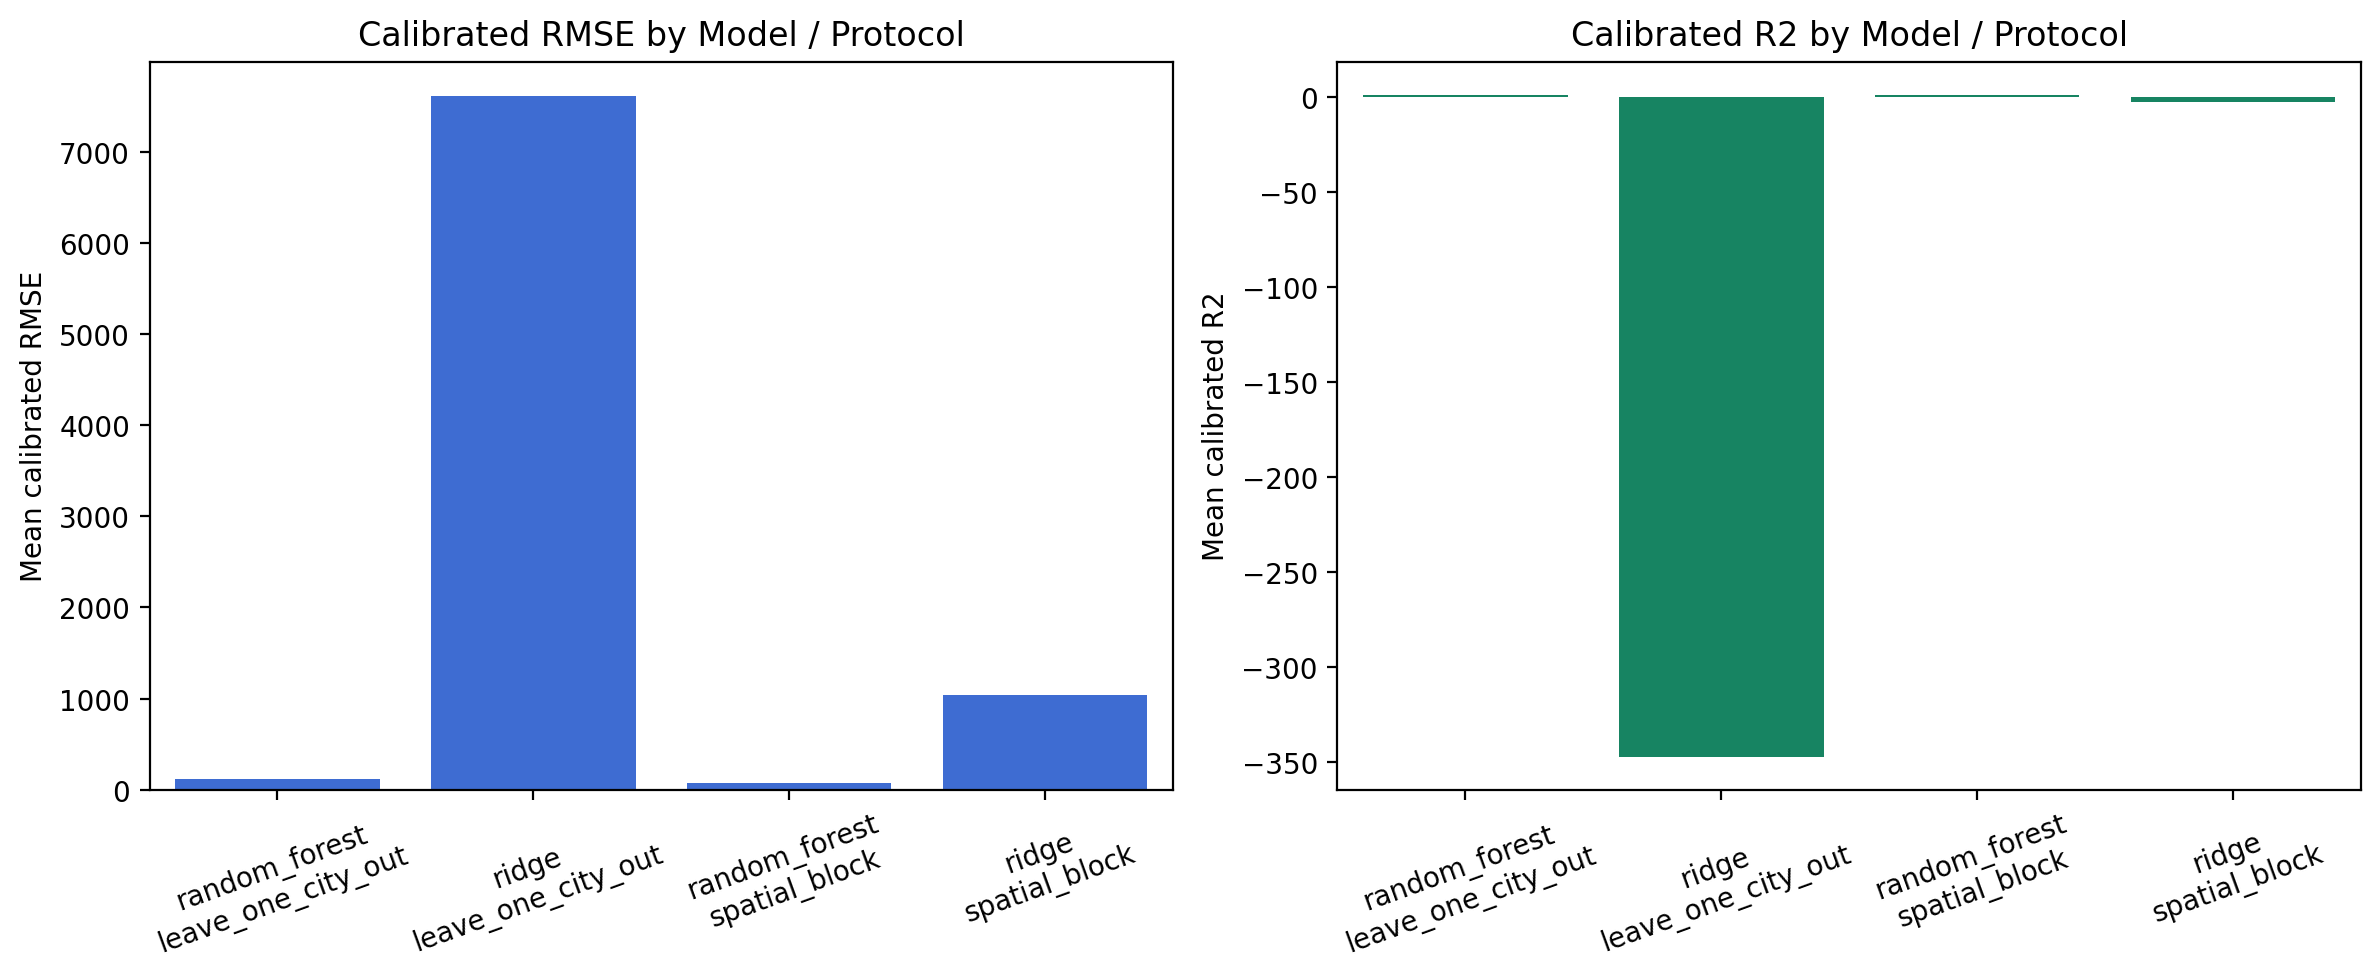
\includegraphics[width=\textwidth]{figures/figure_model_comparison.png}
    \caption{Model comparison}
\end{subfigure}
\hfill
\begin{subfigure}[t]{0.48\textwidth}
    \centering
    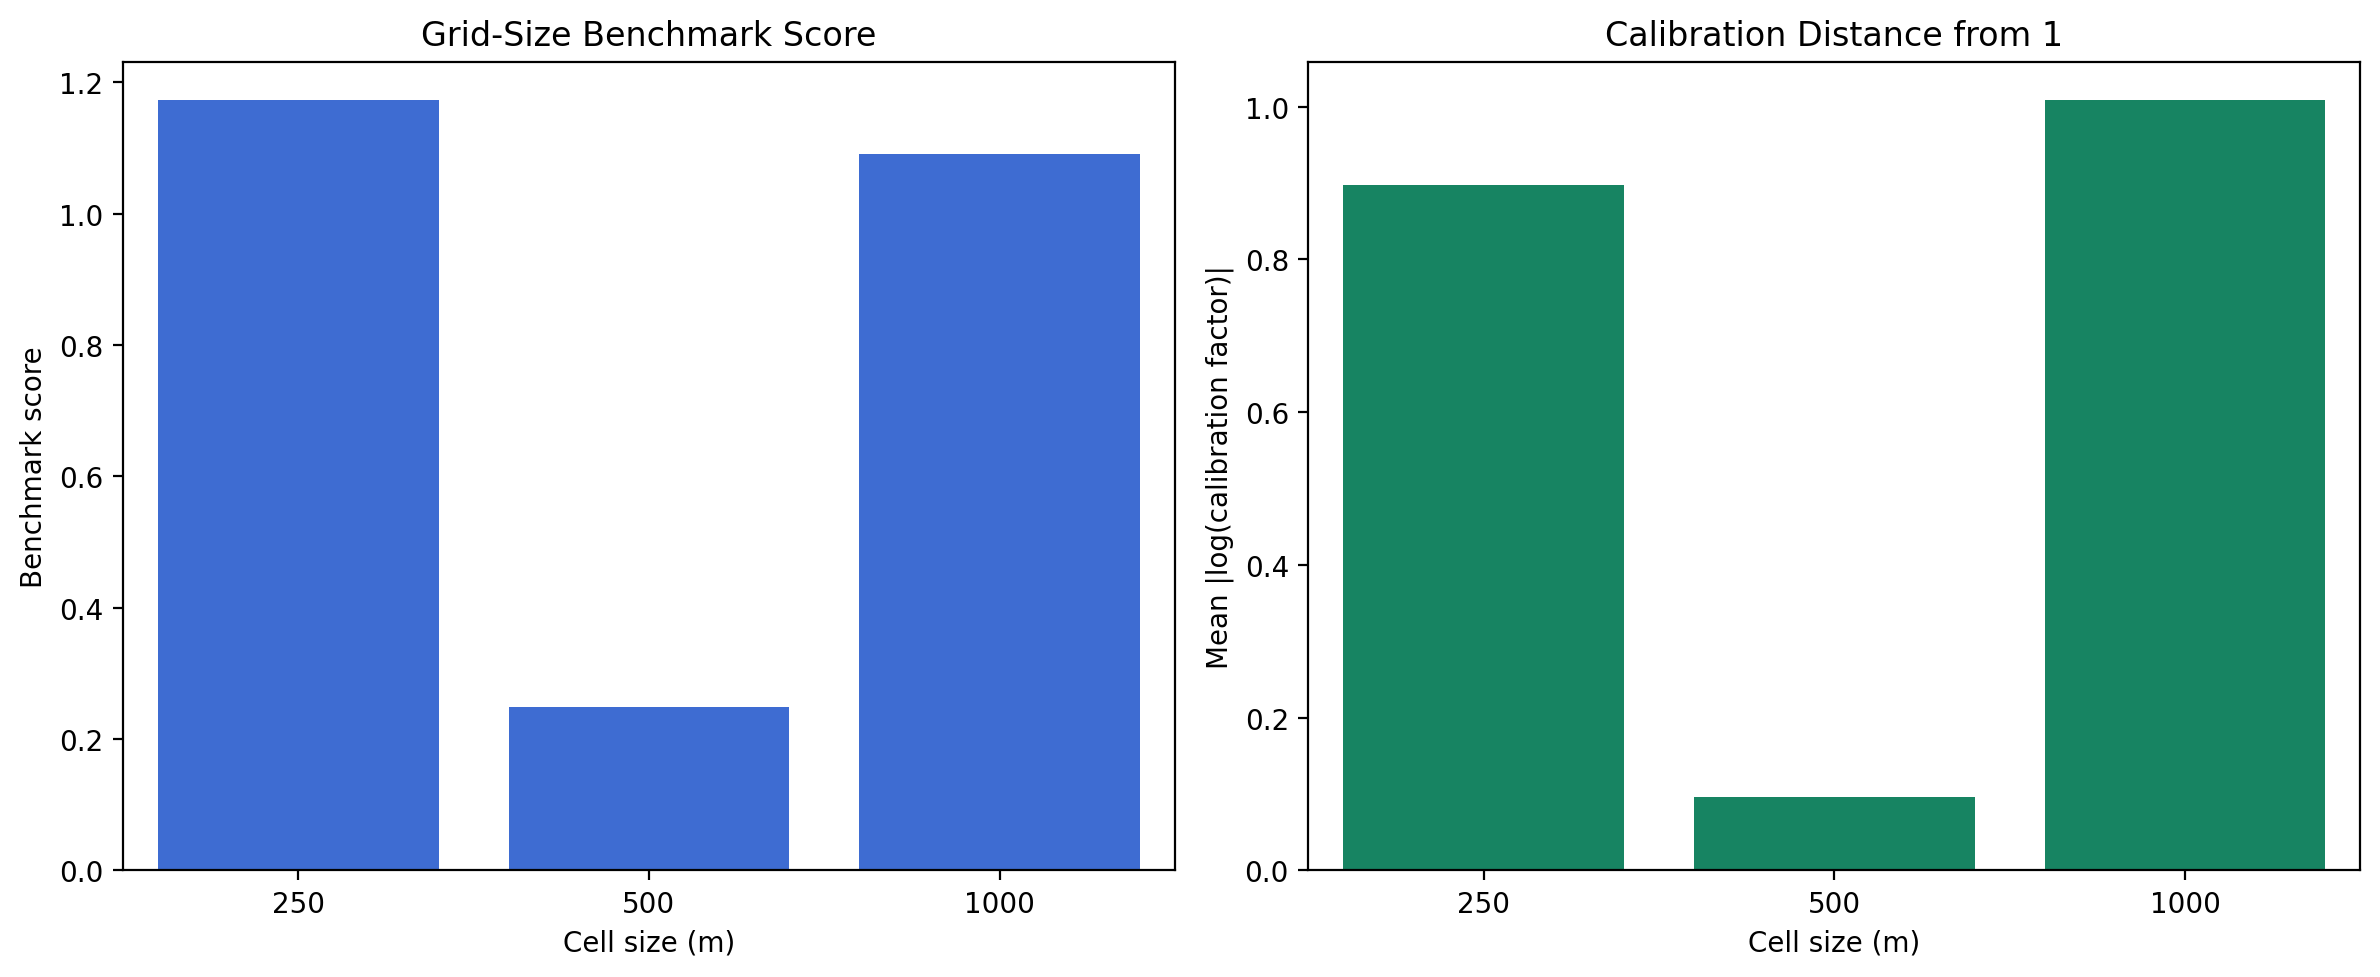
\includegraphics[width=\textwidth]{figures/figure_grid_size_benchmark.png}
    \caption{Grid benchmark}
\end{subfigure}
\caption{Deterministic production selection. Panel (a) shows that Random Forest dominates the ridge comparator under the retained validation protocols. Panel (b) supports 500 m as the fixed production resolution, balancing spatial detail and surface stability.}
\label{fig:deterministic-selection}
\end{figure}

\begin{table}[H]
\centering
\footnotesize
\setlength{\tabcolsep}{4pt}
\renewcommand{\arraystretch}{1.12}
\caption{Core deterministic model and grid validation summary. Calibrated RMSE and calibrated $R^2$ are reported against held-out weak targets after city-level rescaling rather than against observed cell-level census labels.}
\label{tab:core-deterministic-validation}
\begin{adjustbox}{max width=\textwidth}
\begin{tabularx}{\textwidth}{L{1.65cm} Y L{2.10cm} r r r}
\toprule
Component & Setting & Protocol / grid & Calibrated RMSE & Calibrated $R^2$ & Score \\
\midrule
Model & Random Forest & LOCO & 115.934 & 0.934 & -- \\
Model & Ridge & LOCO & 7609.928 & -347.088 & -- \\
Model & Random Forest & spatial block & 76.301 & 0.980 & -- \\
Model & Ridge & spatial block & 1039.817 & -2.690 & -- \\
\midrule
Grid & fixed production choice & 500 m & -- & -- & 0.248572 \\
Grid & finer alternative & 250 m & -- & -- & 1.172821 \\
Grid & coarser alternative & 1000 m & -- & -- & 1.091467 \\
\bottomrule
\end{tabularx}
\end{adjustbox}
\end{table}


\subsection{District benchmark}

District aggregation evidence is strongest in Almaty and weaker in Astana and Shymkent. Almaty reaches Pearson 0.543 and Spearman 0.657 after aggregation, whereas Astana and Shymkent show weak or negative rank-order support. This layer should therefore be interpreted as partial administrative support rather than as truth validation.

The mixed pattern matters because it stops the paper from pretending that district agreement is uniformly strong. Instead, it shows that aggregation can support plausibility where the evidence is good and can remain weak where the support is weaker. That is useful information, but it is not a license to overstate cell-level accuracy.

\begin{figure}[H]
\centering
\begin{subfigure}[t]{0.48\textwidth}
    \centering
    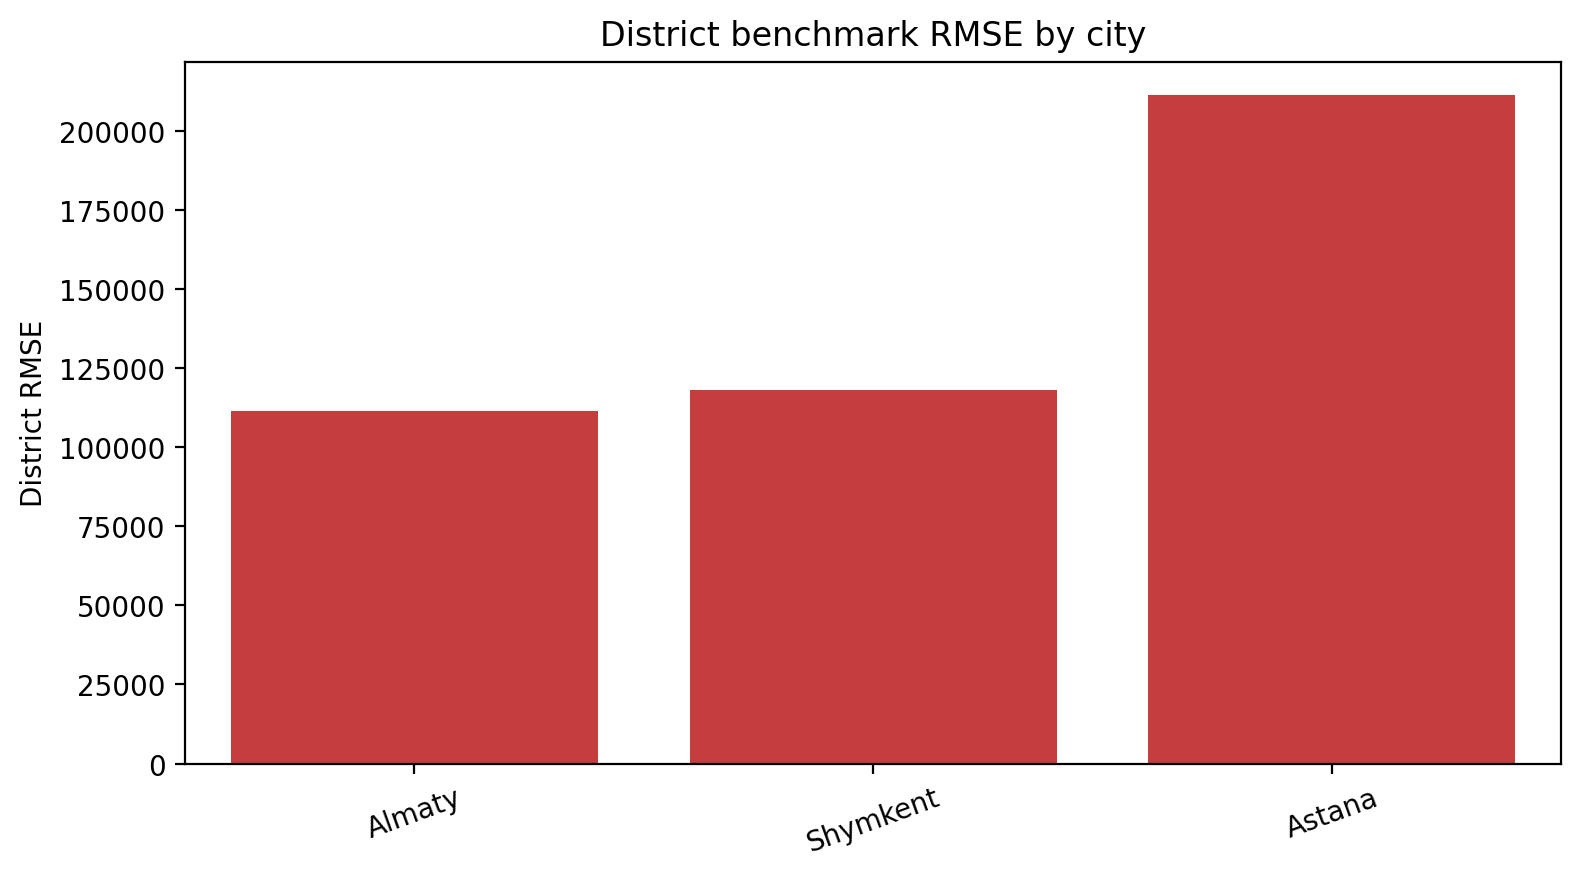
\includegraphics[width=\textwidth]{figures/figure_district_benchmark.png}
    \caption{District benchmark}
\end{subfigure}
\hfill
\begin{subfigure}[t]{0.48\textwidth}
    \centering
    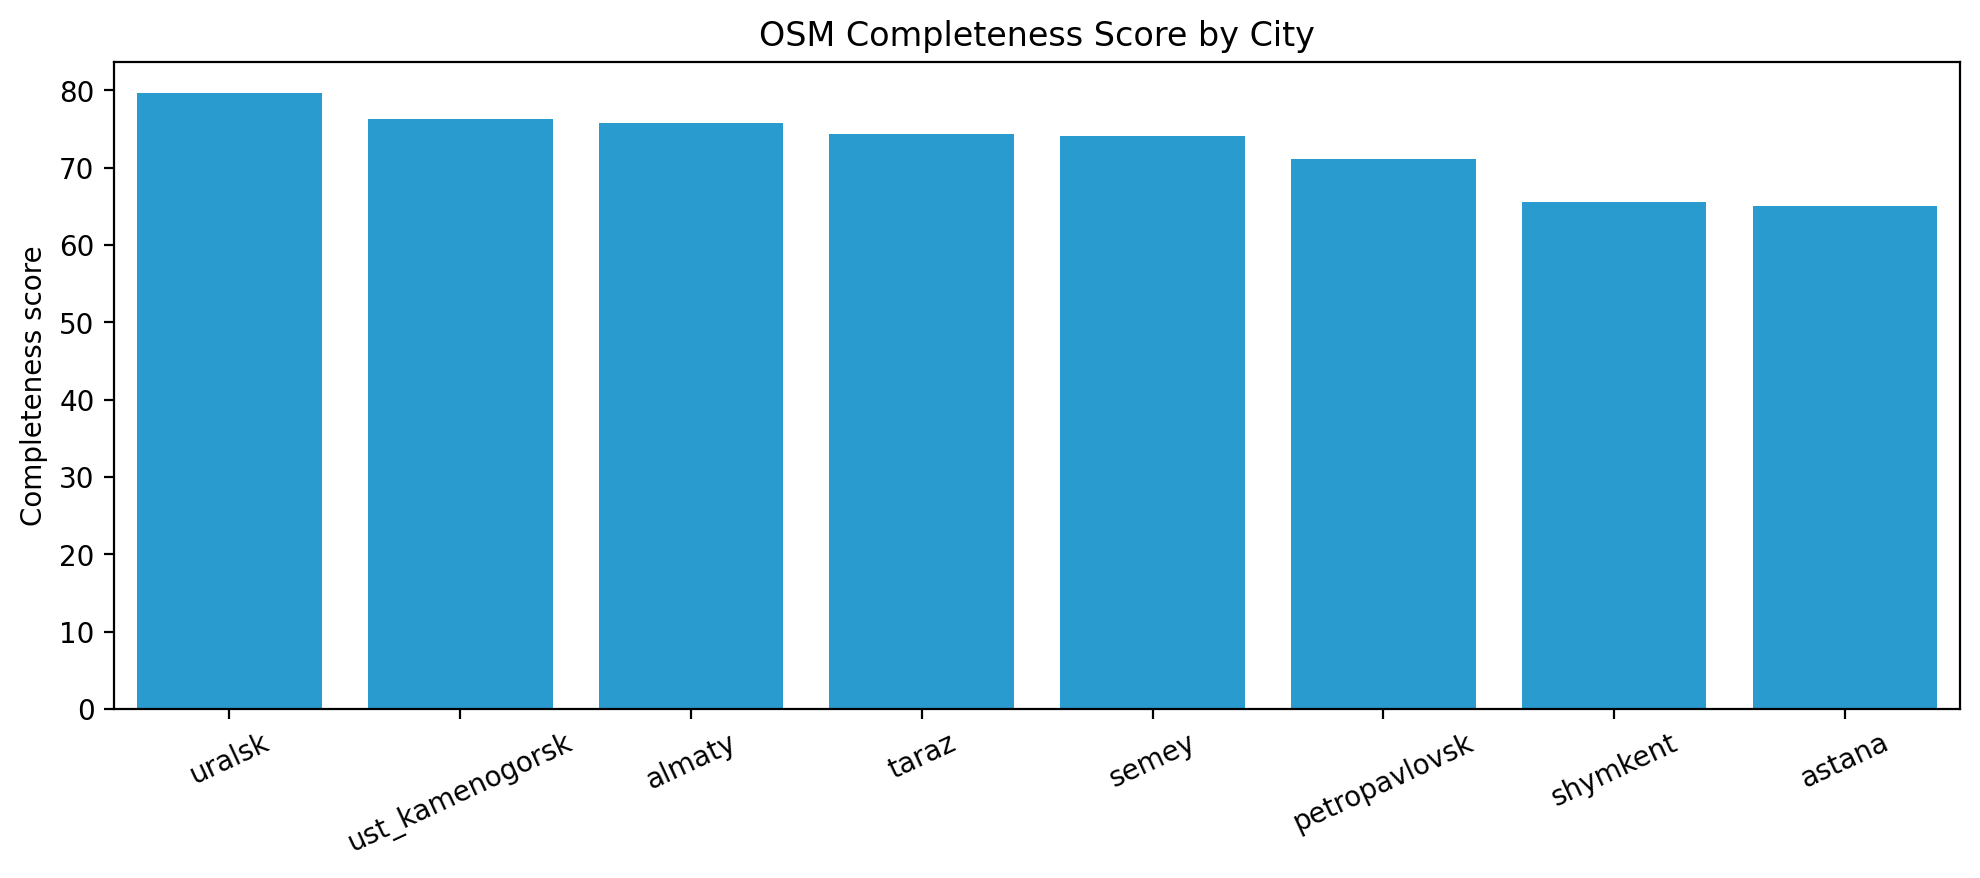
\includegraphics[width=\textwidth]{figures/figure_osm_completeness.png}
    \caption{OSM completeness}
\end{subfigure}
\caption{Internal and support-context evidence for the deterministic baseline. Panel (a) reports district aggregation comparison where administrative references were available. Panel (b) reports OSM completeness, which is used as interpretation context rather than as a direct accuracy metric.}
\label{fig:district-osm}
\end{figure}

\begin{table}[H]
\centering
\caption{Deterministic district benchmark summary. This layer is interpreted as partial administrative support after aggregation rather than as cell-level truth validation.}
\label{tab:district-benchmark-unified}
\begin{tabular}{lrrrrr}
\toprule
City & Compared districts & RMSE & MAPE & Pearson $r$ & Spearman $r$ \\
\midrule
Almaty & 6 & 111379.724 & 37.691 & 0.543 & 0.657 \\
Astana & 5 & 211191.733 & 83.186 & -0.277 & -0.300 \\
Shymkent & 3 & 118069.168 & 42.698 & -0.169 & -0.500 \\
\bottomrule
\end{tabular}
\end{table}



\subsection{External benchmark}

External structural comparison shows complementary support rather than a single winner. WorldPop is strongest for broad correlation, with Pearson 0.877. GHS-POP is strongest for hotspot-sensitive structure, with Spearman 0.834, top-decile overlap 0.614, and hotspot IoU 0.443. This is scientifically useful because it shows that different independent products align with different aspects of the inferred surface.

The interpretation is therefore comparative, not adjudicative. WorldPop helps show whether the surface behaves similarly at a broad spatial level. GHS-POP helps show whether hotspot structure is in the right general place. Neither result means the City1 surface has been validated against truth.

\begin{figure}[H]
\centering
\begin{subfigure}[t]{0.48\textwidth}
    \centering
    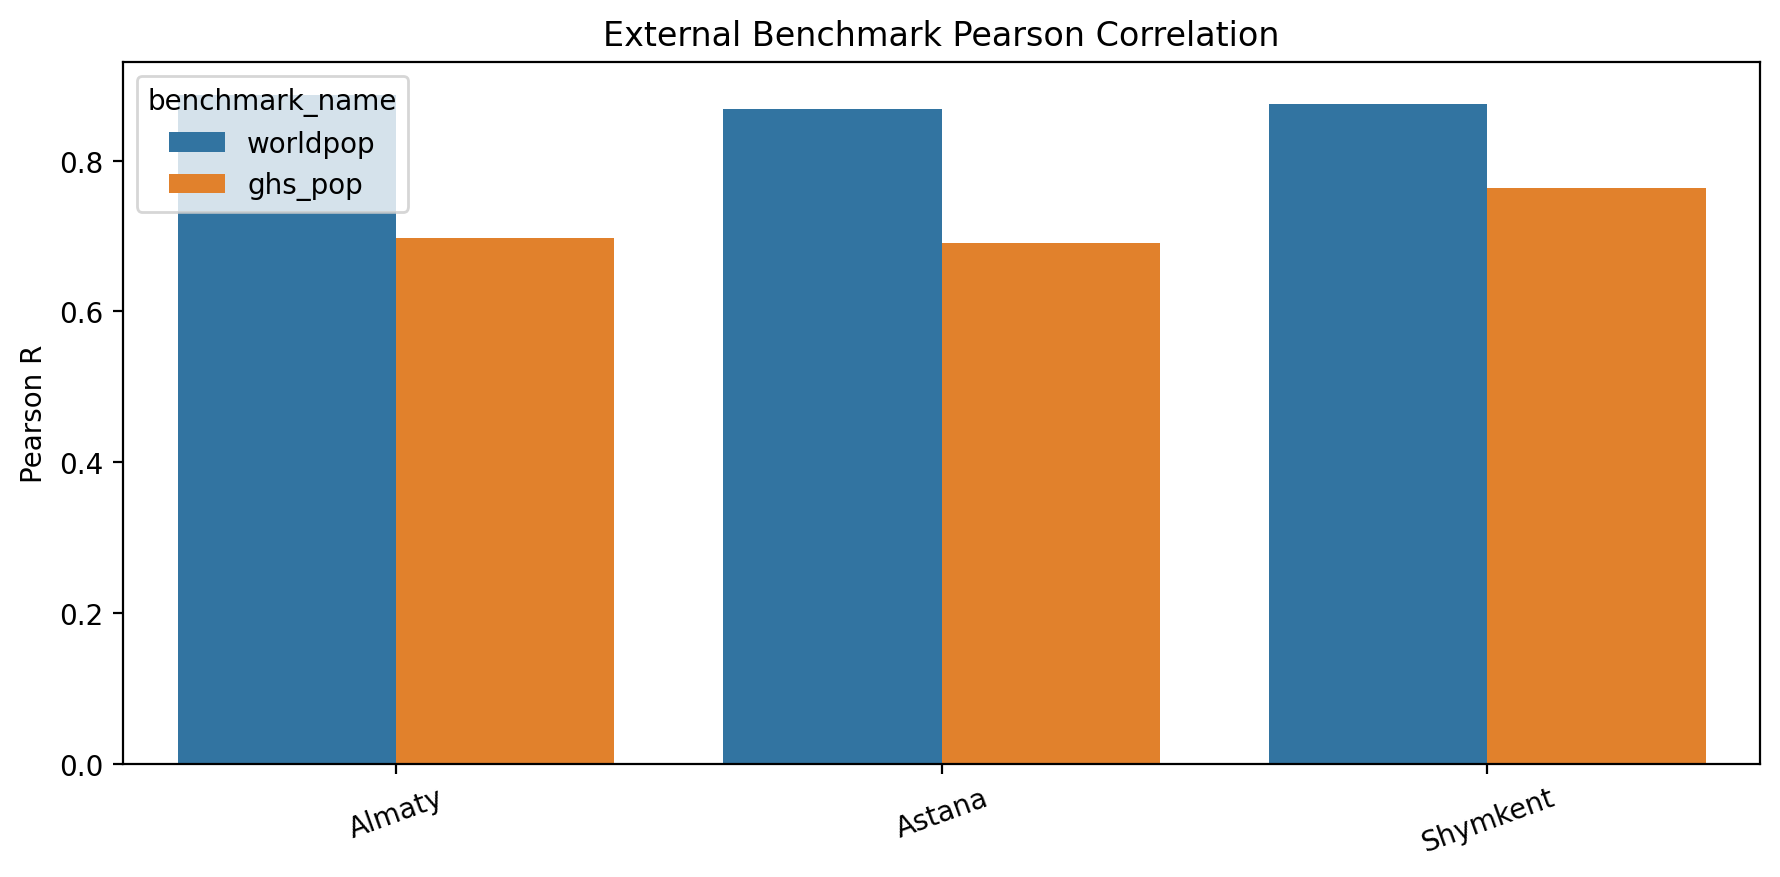
\includegraphics[width=\textwidth]{figures/figure_external_benchmark_pearson.png}
    \caption{Overall correlation}
\end{subfigure}
\hfill
\begin{subfigure}[t]{0.48\textwidth}
    \centering
    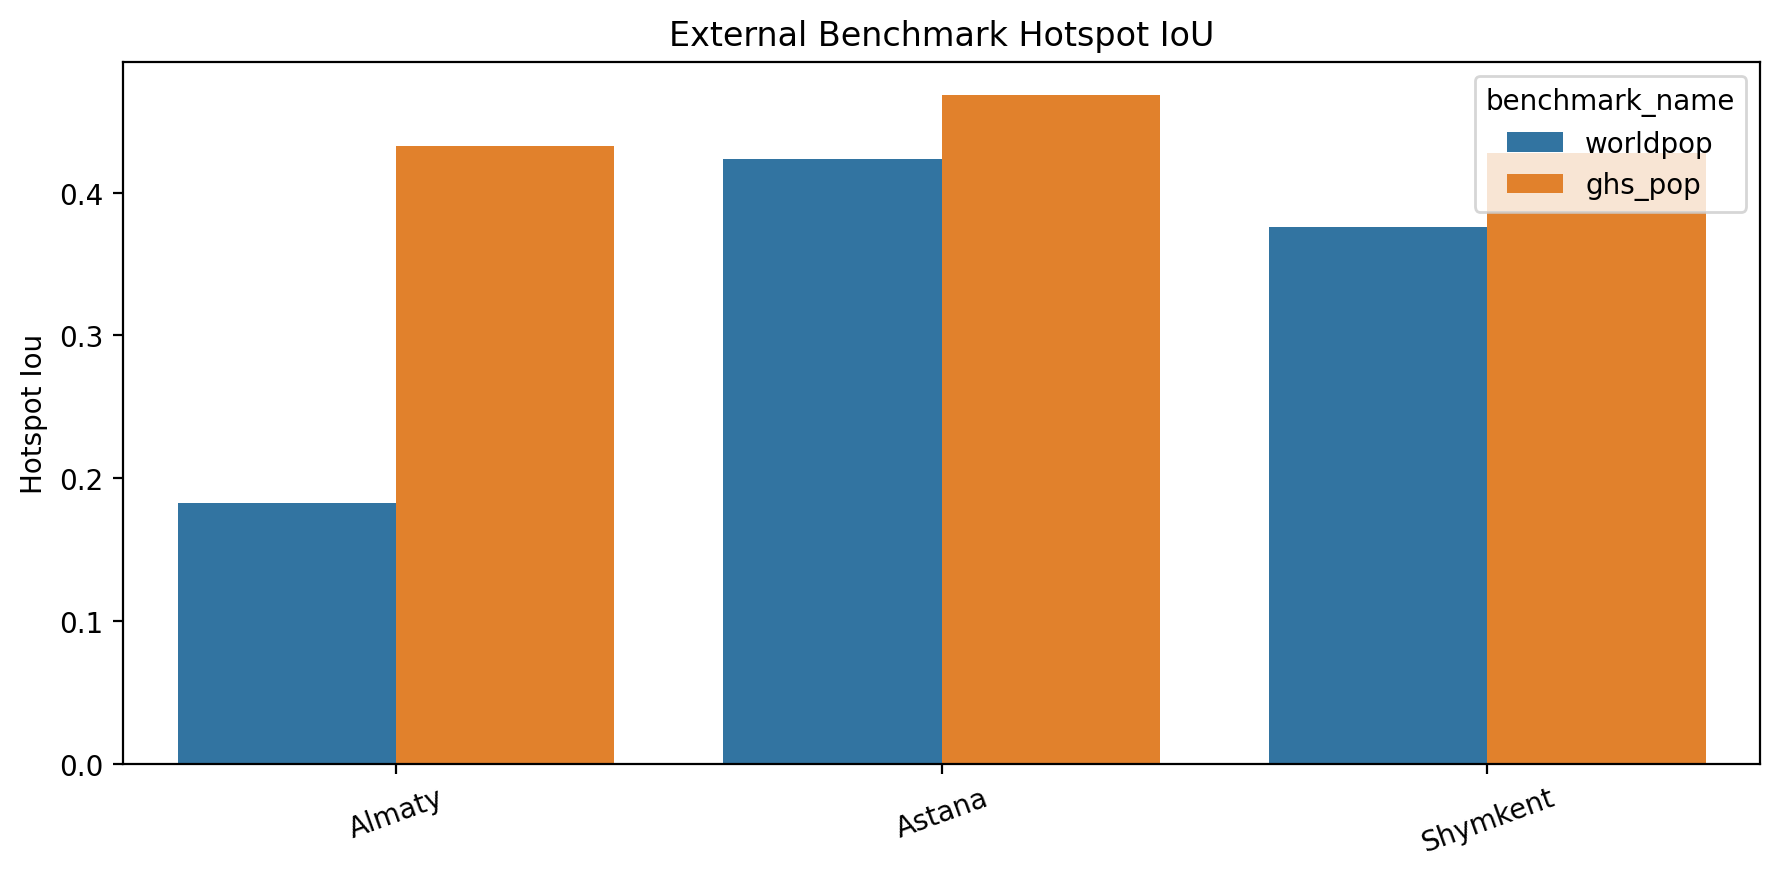
\includegraphics[width=\textwidth]{figures/figure_external_benchmark_hotspot_iou.png}
    \caption{Hotspot-sensitive agreement}
\end{subfigure}
\caption{External structural comparison for the deterministic baseline. WorldPop supports broad structural correlation more strongly, while GHS-POP supports hotspot-sensitive agreement more strongly. These are structural comparators rather than ground truth.}
\label{fig:external-structure}
\end{figure}

\begin{table}[H]
\centering
\caption{Deterministic external benchmark summary from independent gridded population products. These comparisons are used as structural agreement checks rather than as direct truth validation.}
\label{tab:external-benchmark-unified}
\begin{tabular}{lrrrr}
\toprule
Benchmark & Pearson $r$ & Spearman $r$ & Top-decile overlap & Hotspot IoU \\
\midrule
WorldPop & 0.877 & 0.831 & 0.483 & 0.327 \\
GHS-POP & 0.718 & 0.834 & 0.614 & 0.443 \\
\bottomrule
\end{tabular}
\end{table}



\subsection{Ablation}

The full feature set remains strongest overall, while built-form-only is the strongest reduced predictor family. The full feature configuration achieves a calibrated RMSE of 115.934 and calibrated $R^2$ of 0.934. Built-form-only remains close behind at calibrated RMSE 120.656 and calibrated $R^2$ 0.929, while transport-only and POI/services-only are much weaker. Calibration also materially improves the final output, with a full-model RMSE gain of 135.821 between raw and calibrated outputs.

The ablation story is important because it reveals the core signal family without reducing the paper to a single feature-engineering trick. Built form carries the dominant reduced-family signal, which is intuitive for urban population allocation, but the full stack remains strongest because the city surface is shaped by multiple types of open-data evidence at once. That combination is what makes the calibrated proxy surface more credible than any one family alone.

\input{tables_tex/table6_ablation_summary.tex}

\subsection{Qualitative plausibility}

Qualitative plausibility is locked to Almaty and Astana. In both cities, dense residential and central mixed-use zones tend to receive higher predicted population, while peripheral open or weak-built zones tend to remain low. Almaty provides the stronger completeness case and therefore the stronger visual plausibility reading. Astana remains more cautious but still preserves interpretable urban morphology. This layer supports plausibility, not cell-level truth.

The qualitative reading is intentionally modest. It does not say the map is “correct”; it says the map is consistent with visible urban structure in a way that supports the bounded proxy claim. That is exactly the kind of evidence a reviewer expects when the paper cannot rely on true cell-level census labels.

\begin{figure}[H]
\centering
\begin{subfigure}[t]{0.49\textwidth}
    \centering
    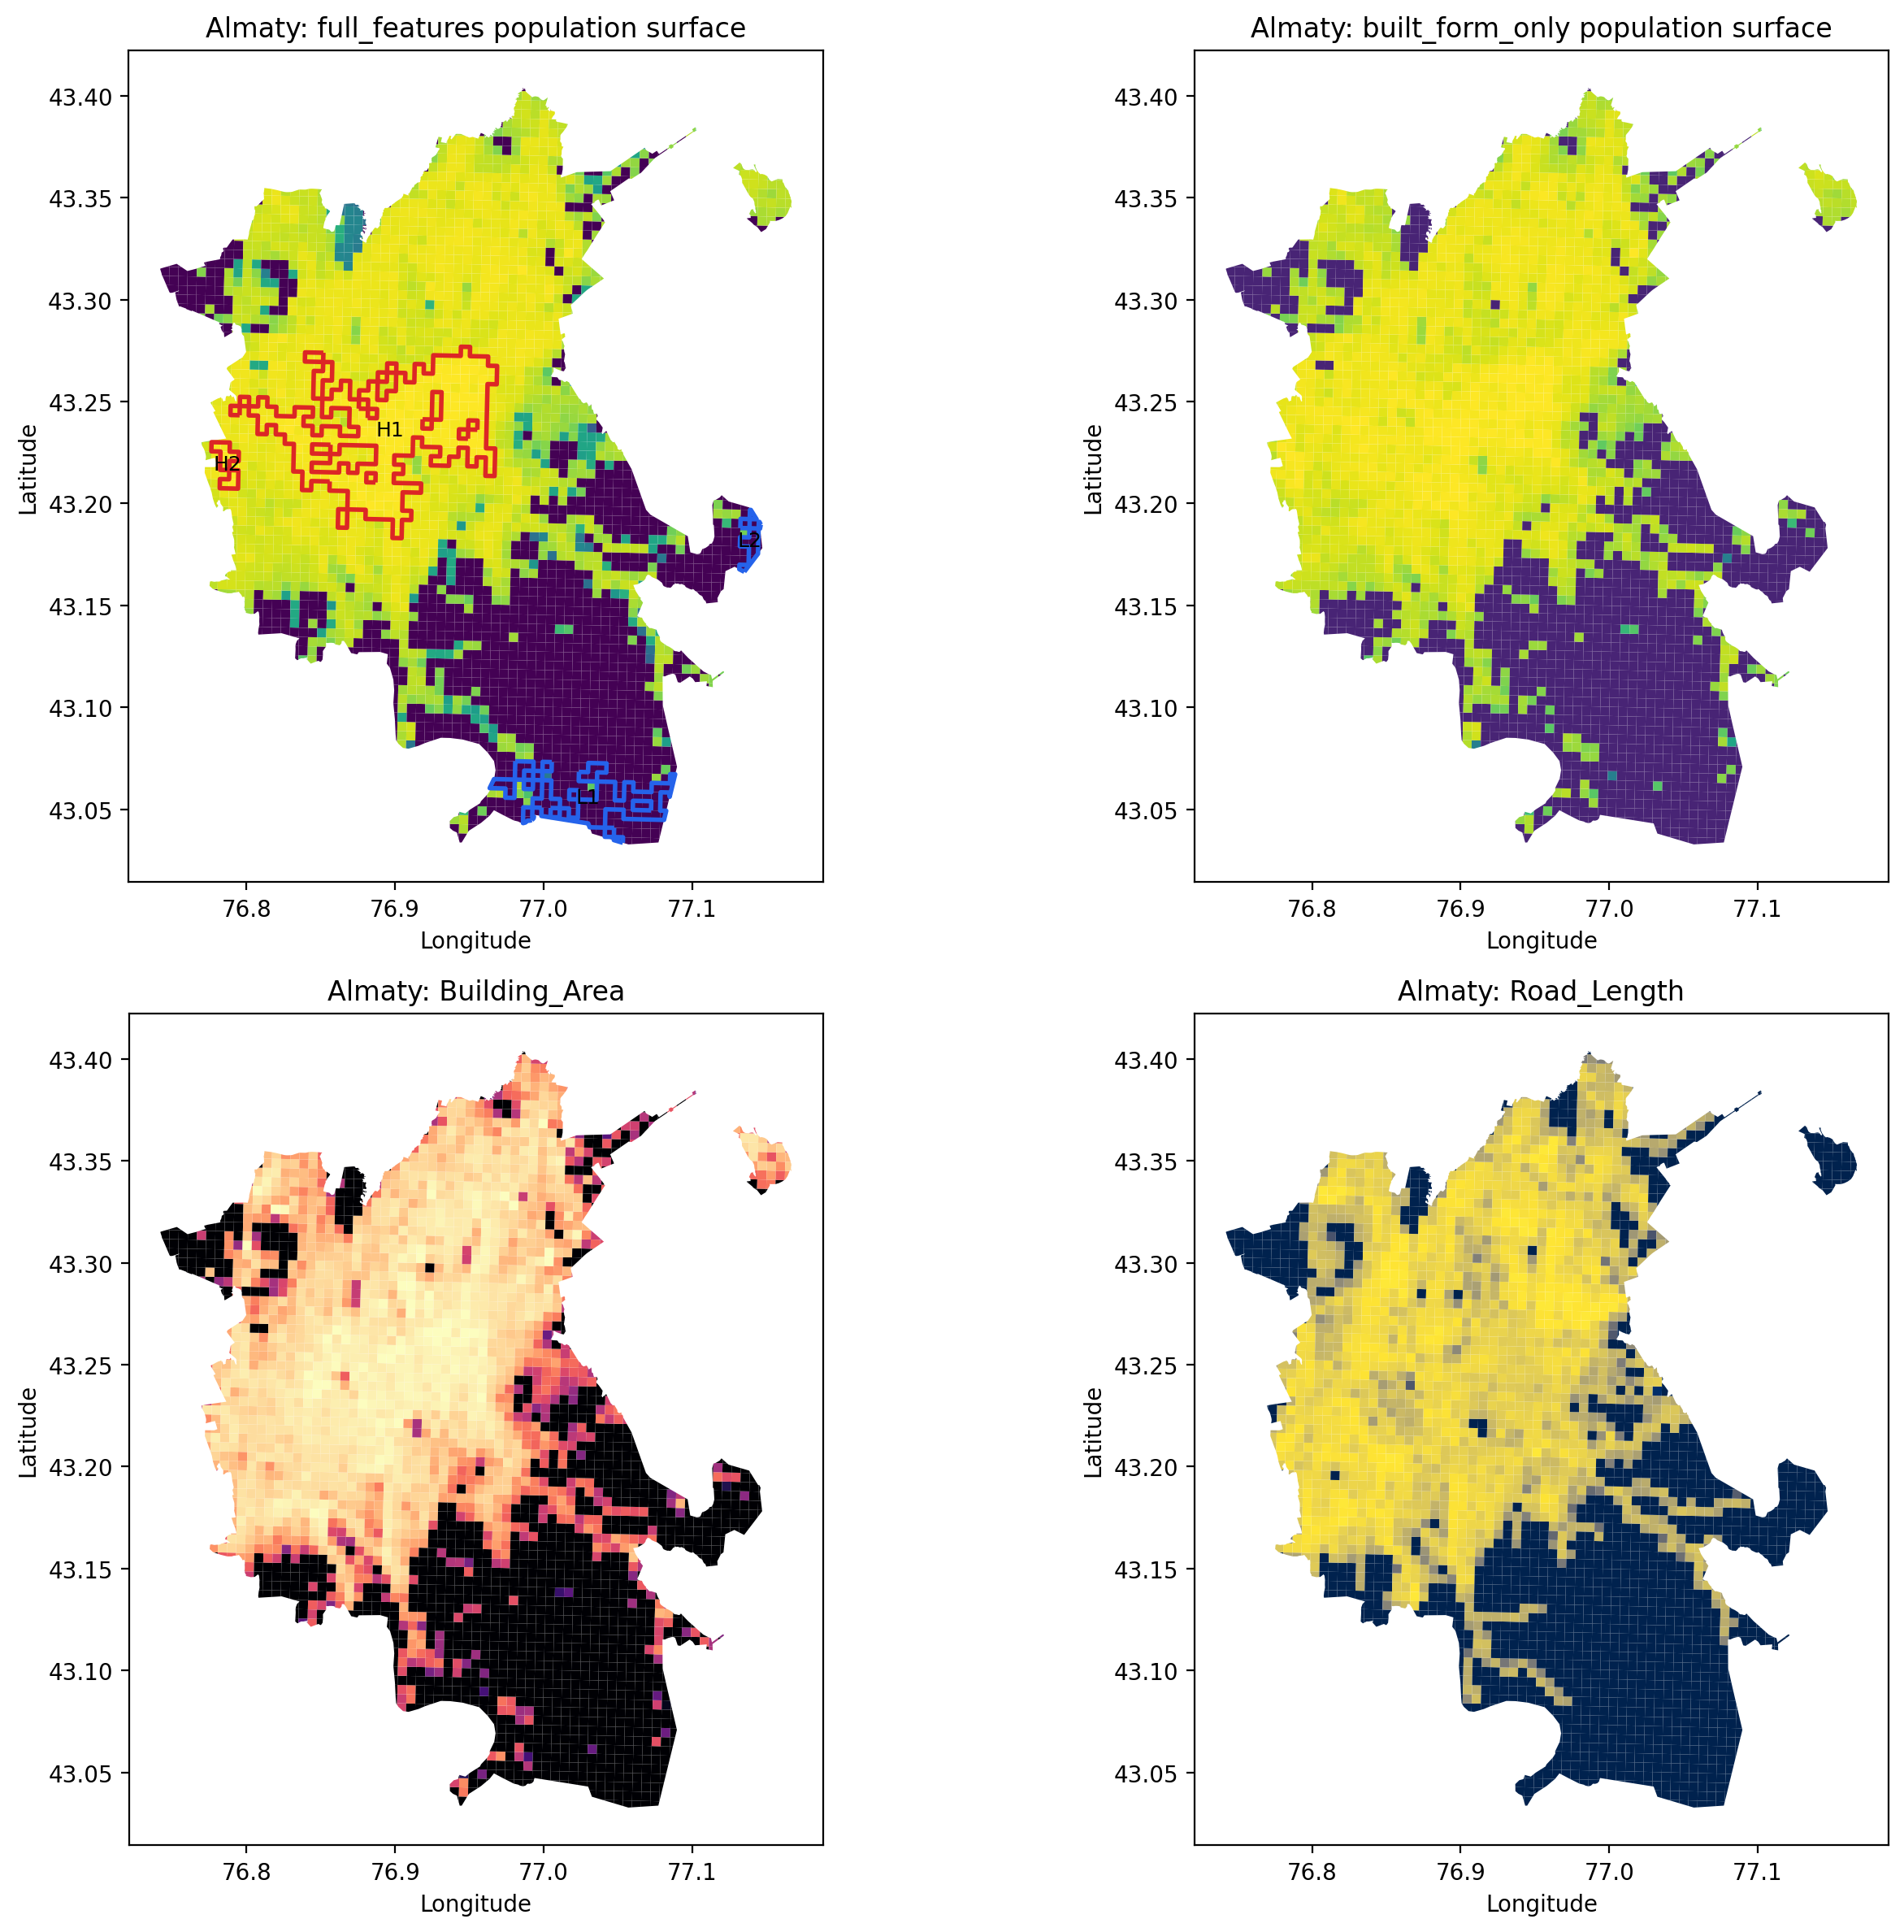
\includegraphics[width=\textwidth]{figures/figure_qualitative_overview_almaty.png}
    \caption{Almaty overview}
\end{subfigure}
\hfill
\begin{subfigure}[t]{0.49\textwidth}
    \centering
    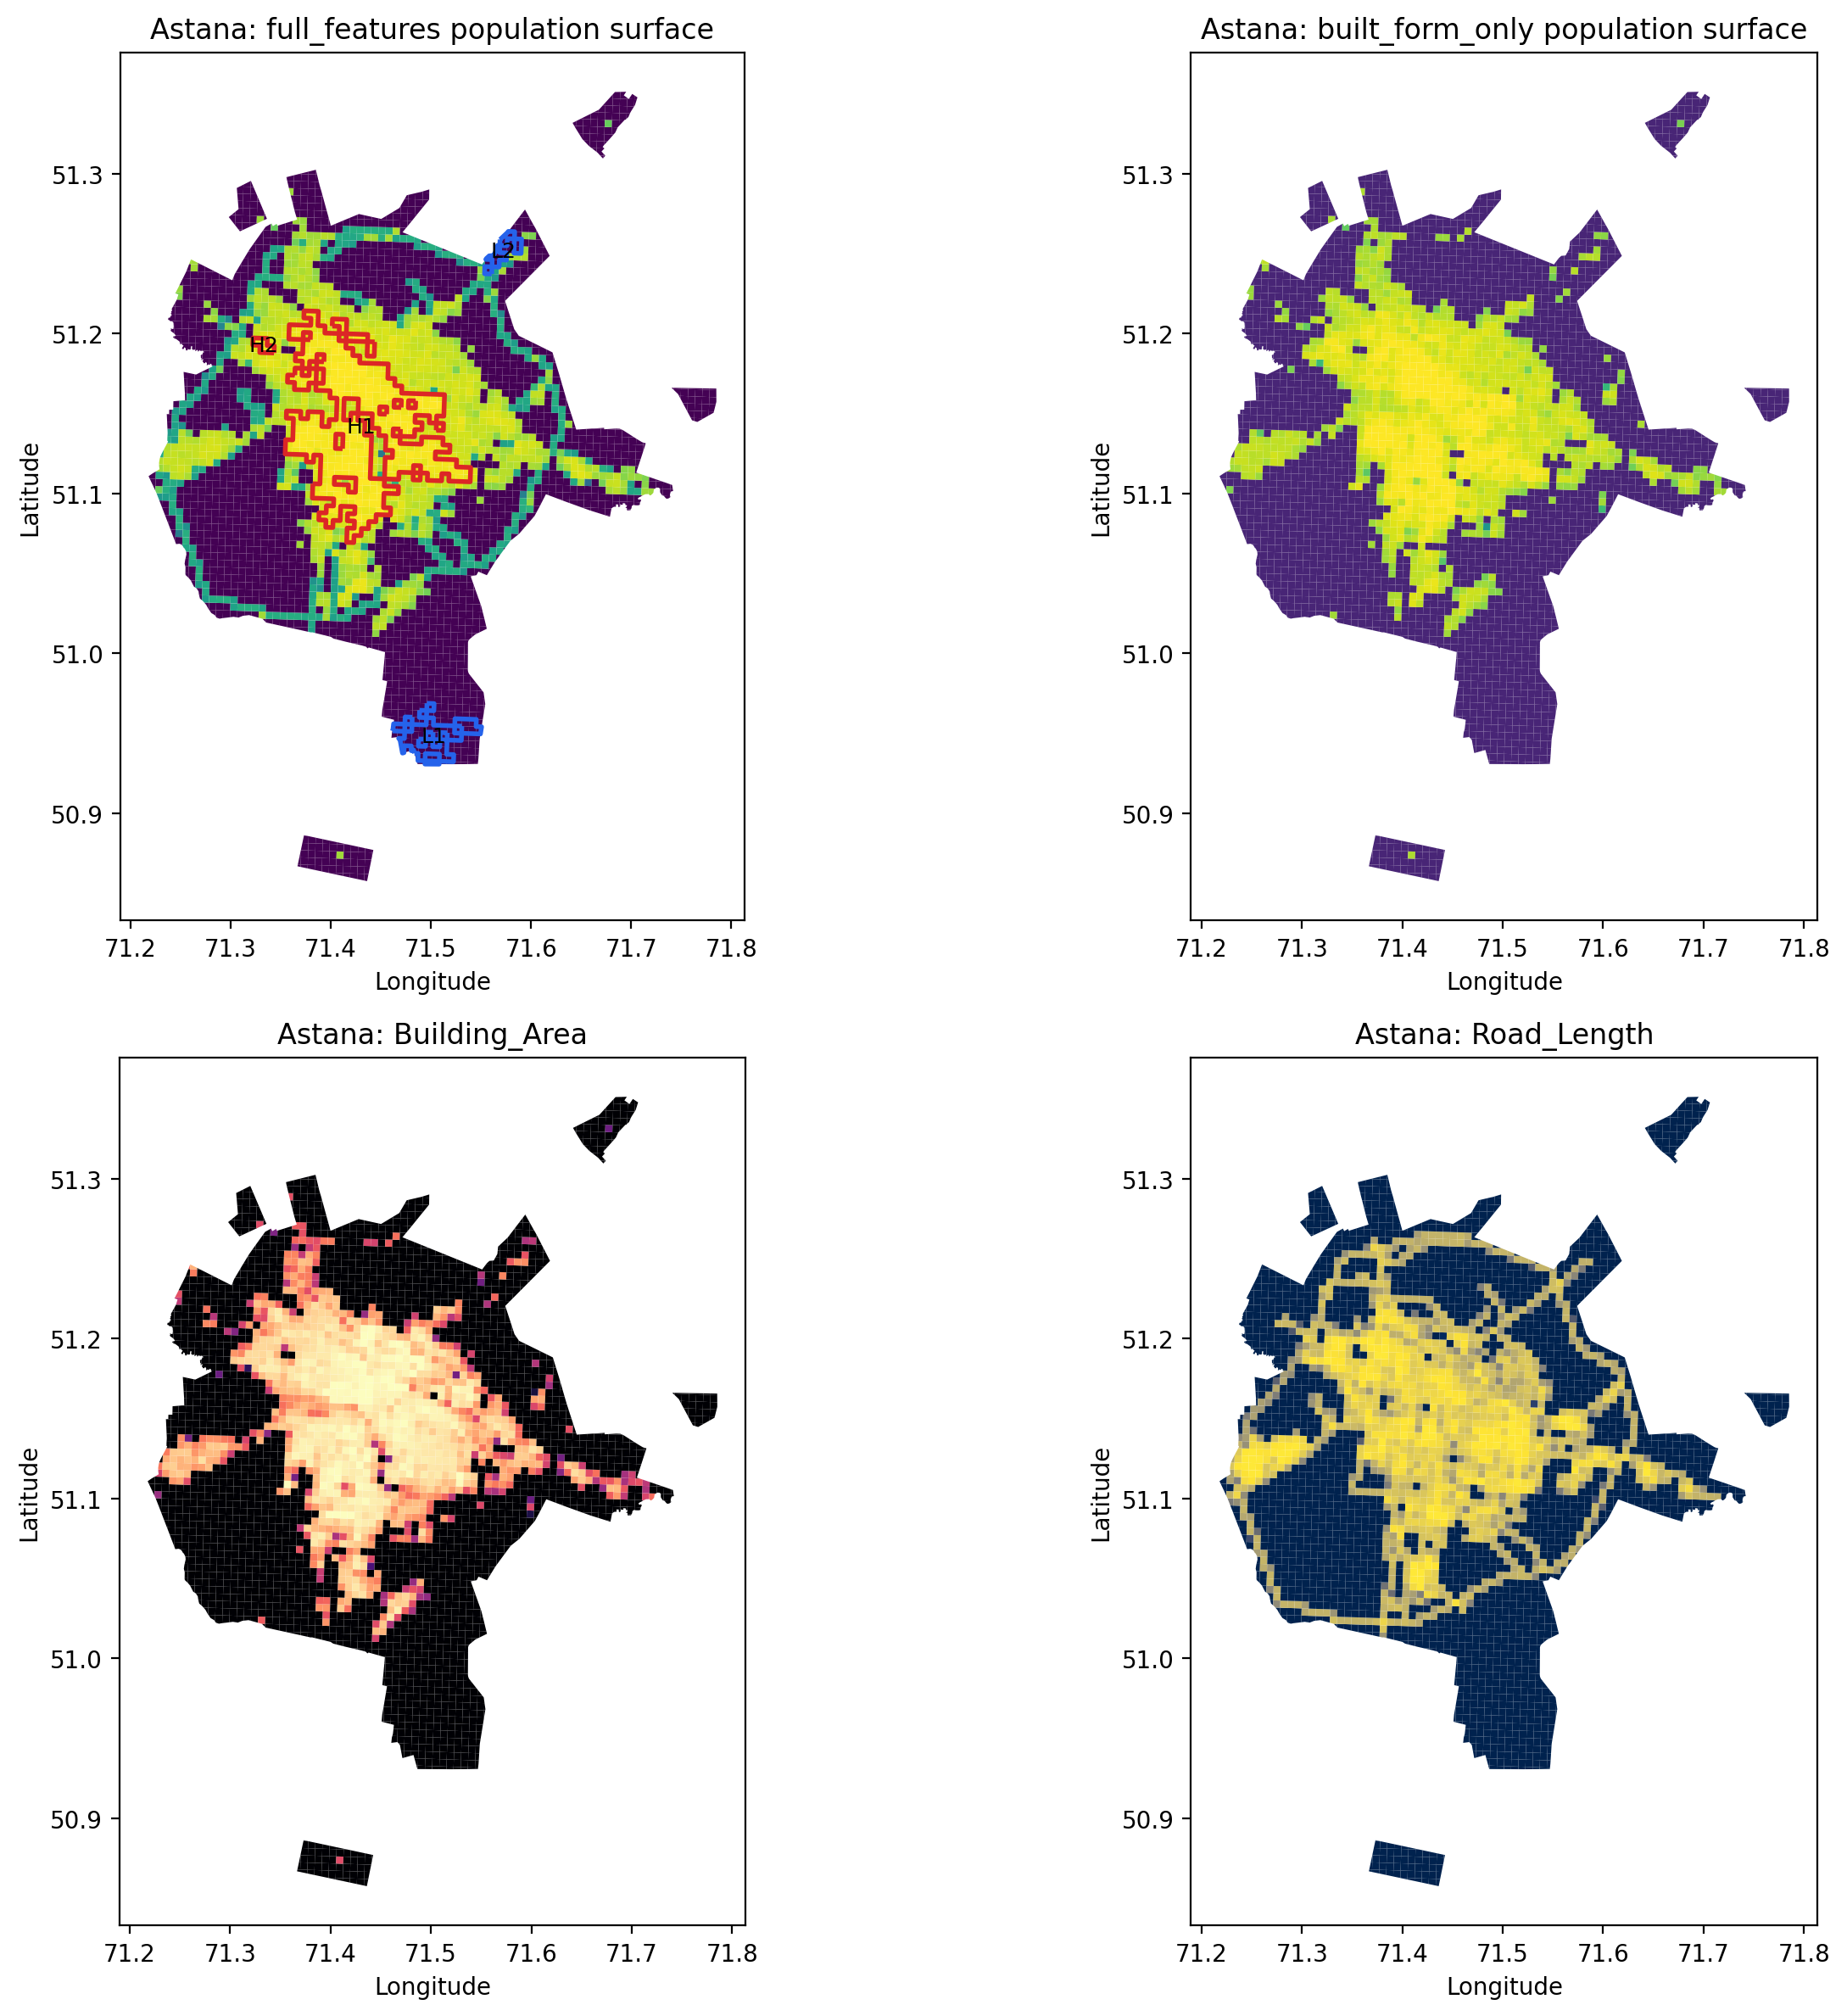
\includegraphics[width=\textwidth]{figures/figure_qualitative_overview_astana.png}
    \caption{Astana overview}
\end{subfigure}
\caption{Qualitative plausibility overview for the deterministic baseline. The maps compare the calibrated proxy surface with visible built-environment structure and are interpreted as urban-structural plausibility evidence rather than as truth validation.}
\label{fig:qualitative-overview-unified}
\end{figure}

\section{Results II: Reliability, Uncertainty, and Hotspot Use}

\subsection{City coverage and uncertainty outputs}

The uncertainty-aware inference package covers Almaty, Astana, Semey, and Shymkent. By construction, the calibrated median surface sums to the official total in every city. What varies is the uncertainty burden and confidence structure. Almaty has the lowest median relative uncertainty (0.170) and the largest high-confidence share (22.9\%). Semey has the highest median relative uncertainty (0.349) but still retains a small high-confidence subset (3.4\%). Astana and Shymkent are more caution-heavy and retain no high-confidence share in the reference city summary.

This city contrast is the first hint that Stage 2 is doing real interpretive work. The same calibrated proxy framework behaves differently depending on support conditions, and that difference is precisely what the uncertainty layer is designed to expose.

\begin{table}[H]
\centering
\small
\caption{Uncertainty-aware city coverage summary. The calibrated median surface sums to the official total in every city by construction. Confidence shares are reported as percentages of city cells.}
\label{tab:uncertainty-city-coverage-unified}
\begin{tabular}{lrrrrrrl}
\toprule
City & Cells & Official total & Median rel.\ unc. & High (\%) & Medium (\%) & Low (\%) & OSM label \\
\midrule
Almaty   & 3078 & 2351424 & 0.170 & 22.9 & 66.2 & 10.9 & good \\
Astana   & 3473 & 1649242 & 0.281 & 0.0  & 63.7 & 36.3 & moderate \\
Semey    & 1033 & 315382  & 0.349 & 3.4  & 79.7 & 16.9 & good \\
Shymkent & 4939 & 1298279 & 0.175 & 0.0  & 69.9 & 30.1 & moderate \\
\bottomrule
\end{tabular}
\end{table}



\begin{figure}[H]
\centering
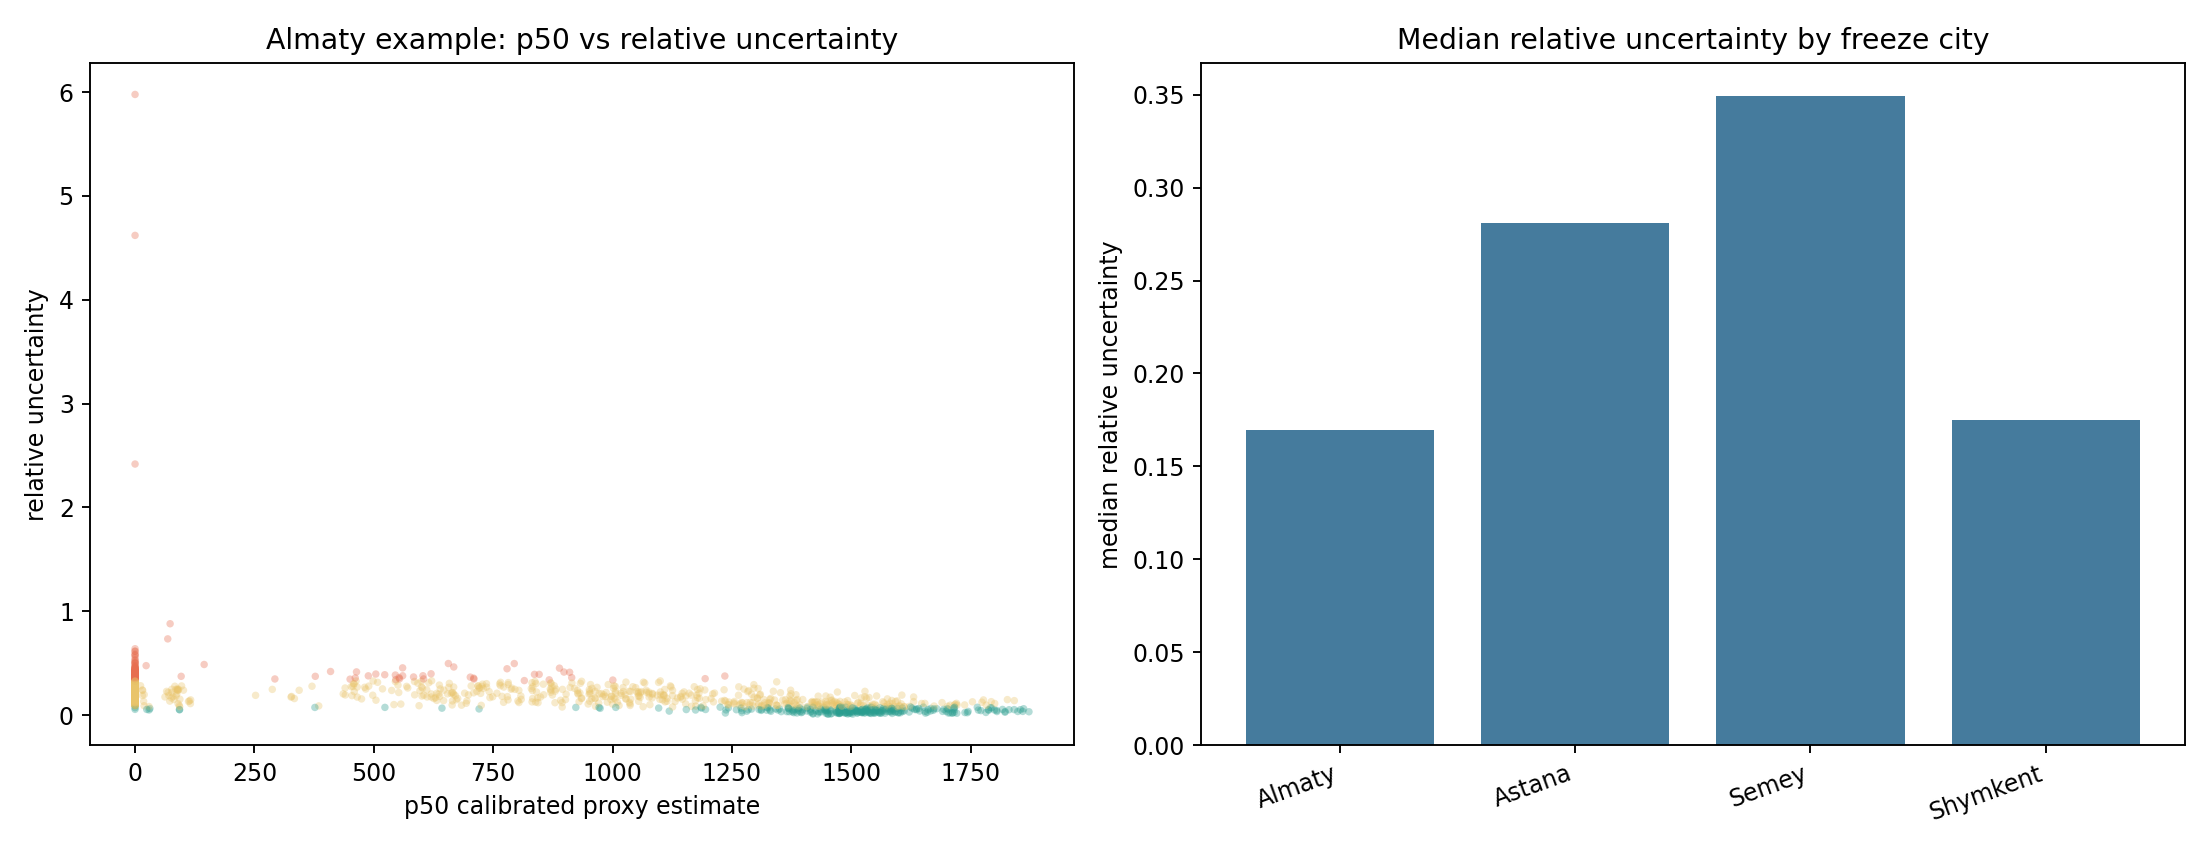
\includegraphics[width=\textwidth]{figures/fig2_uncertainty_output_example.png}
\caption{Uncertainty output summary. Left: Almaty calibrated median proxy estimates against relative uncertainty. Right: median relative uncertainty by city. The figure shows that uncertainty burden varies within and across cities, but it does not estimate true census uncertainty.}
\label{fig:uncertainty-output-unified}
\end{figure}

\subsection{Confidence-band distribution}

Confidence bands separate stronger and weaker interpretation contexts across the four-city package. Almaty is the clearest high-confidence case. Semey retains only a small high-confidence share. Astana and Shymkent are dominated by medium and low bands. These bands are interpretation support classes, not correctness probabilities.

The band separation is useful because it allows the same surface to be read differently in different cities without pretending that one summary number applies everywhere. This is the practical value of the confidence layer: it changes how the map should be used, even when the underlying median surface is unchanged.

\begin{figure}[H]
\centering
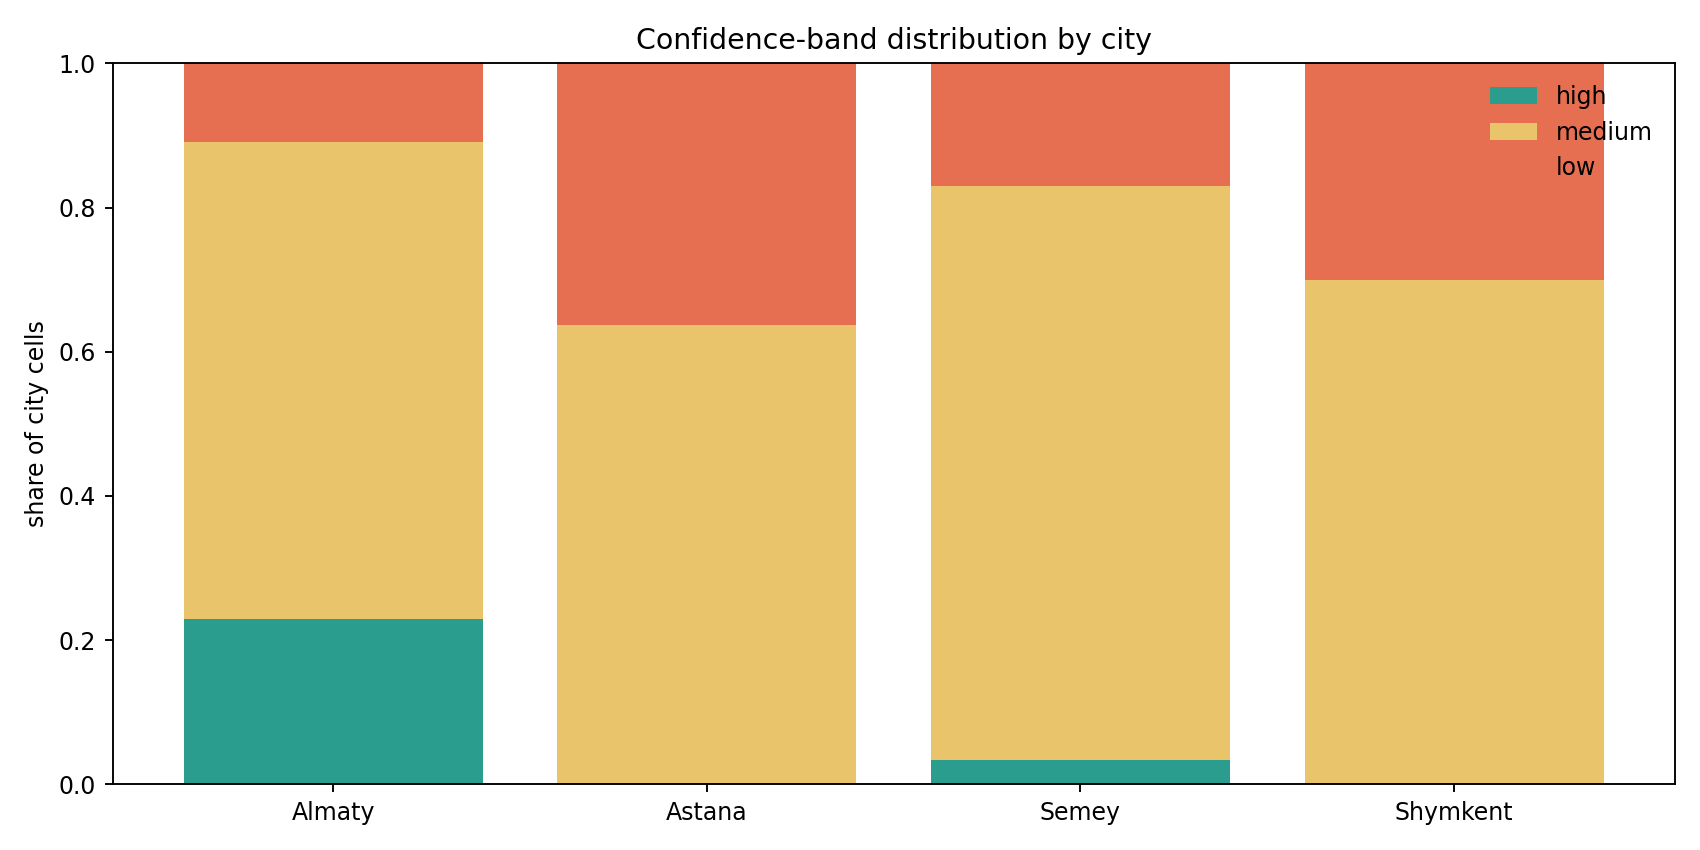
\includegraphics[width=0.95\textwidth]{figures/fig3_confidence_band_distribution.png}
\caption{Confidence-band distribution by city. The figure highlights where the calibrated proxy surface can be read more assertively for screening and where it should be treated more cautiously.}
\label{fig:confidence-distribution-unified}
\end{figure}

\subsection{Hotspot prioritization}

Hotspot prioritization translates the uncertainty layer into a bounded practical use case. Almaty is the strongest stable hotspot-screening case, with 212 \texttt{high\_value\_high\_confidence} cells and 310 \texttt{medium\_value\_high\_confidence} cells. Semey is mixed, retaining a small stable high-value subset but also a larger caution-heavy tail. Astana and Shymkent are dominated by review-oriented classes.

This is the clearest applied output of Stage 2. The framework is not saying that these are verified hotspots. It is saying that some hotspots are better supported for screening and triage than others, which is exactly the kind of distinction planners and analysts need when the evidence base is incomplete.

\begin{table}[H]
\centering
\small
\setlength{\tabcolsep}{4pt}
\renewcommand{\arraystretch}{1.08}
\caption{Hotspot prioritization summary by city. Stable high-value classes are concentrated in Almaty, whereas Astana and Shymkent are dominated by review-oriented classes.}
\label{tab:hotspot-priority-unified}
\resizebox{\textwidth}{!}{%
\begin{tabular}{lrrrrrrr}
\toprule
City & Priority cells & High/high & High/low & Medium/high & Low/high-unc. & Mean conf. & Median rel.\ unc. \\
\midrule
Almaty   & 842  & 212 & 0  & 310 & 320  & 0.609 & 0.060 \\
Astana   & 712  & 0   & 4  & 0   & 708  & 0.328 & 0.423 \\
Semey    & 169  & 4   & 19 & 10  & 136  & 0.397 & 0.591 \\
Shymkent & 1256 & 0   & 89 & 0   & 1167 & 0.323 & 0.312 \\
\bottomrule
\end{tabular}
}
\end{table}


\begin{figure}[H]
\centering
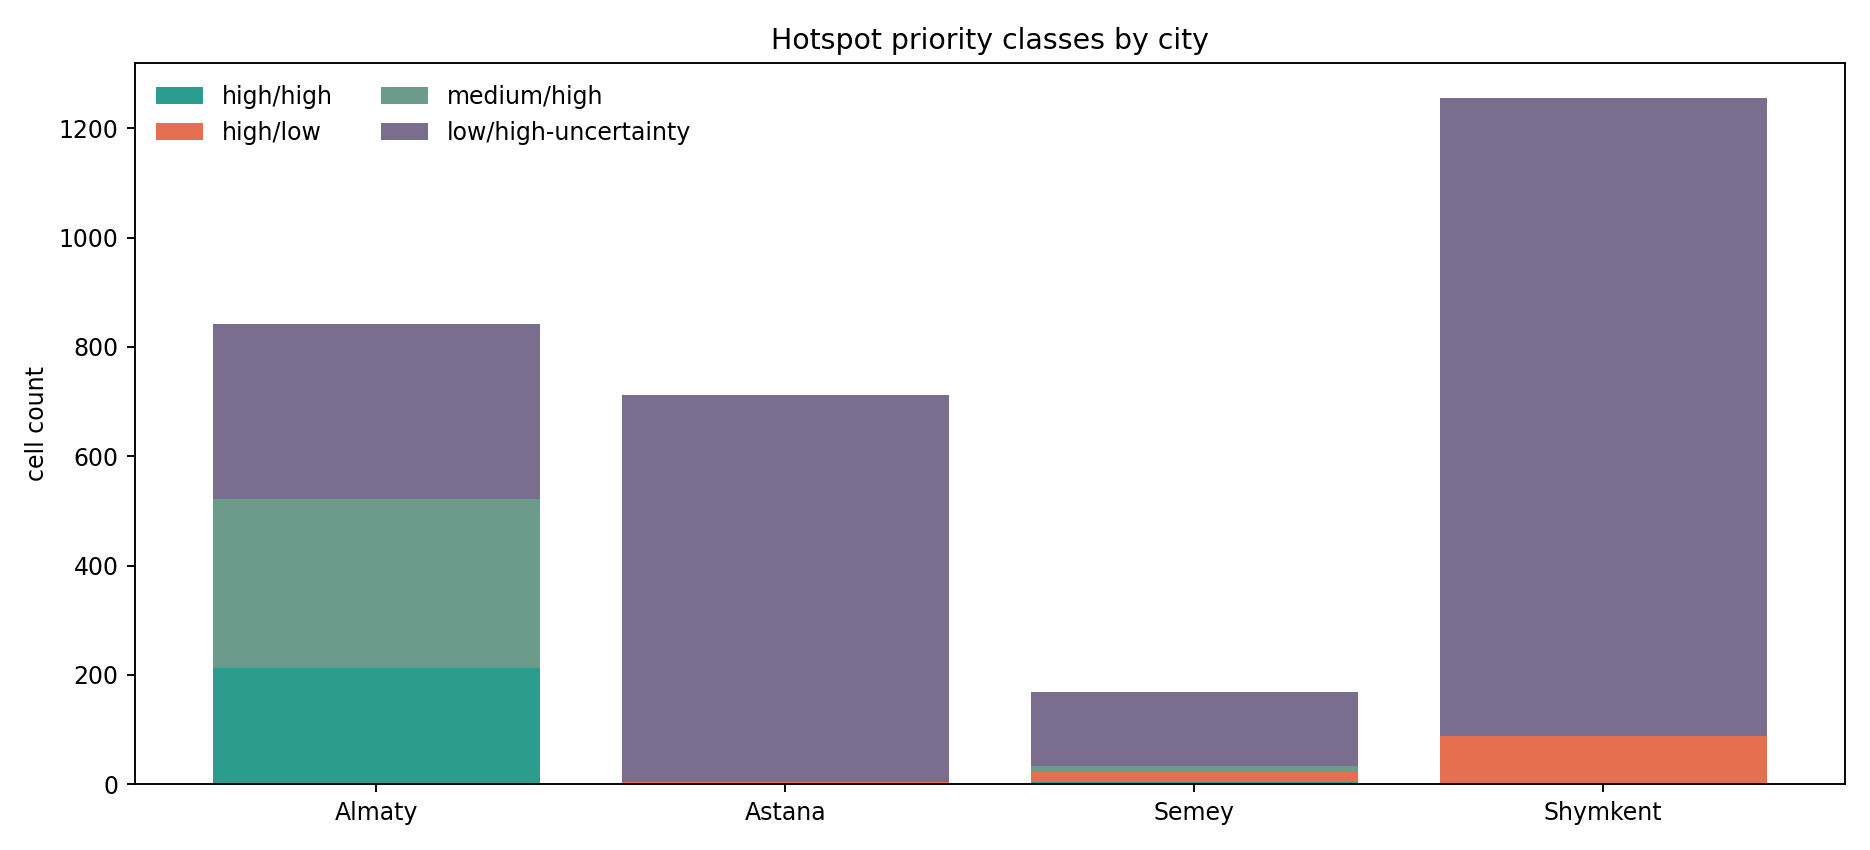
\includegraphics[width=0.95\textwidth]{figures/fig4_hotspot_prioritization_by_city.png}
\caption{Hotspot priority classes by city. Almaty concentrates the strongest stable hotspot support, whereas Astana and Shymkent are dominated by caution-oriented classes. These are screening classes rather than verified hotspot truth.}
\label{fig:hotspot-priority-unified}
\end{figure}

\subsection{Interval coverage and error alignment}

Interval coverage is mixed rather than uniformly strong. Under the bounded LOCO-like protocol, coverage ranges from 0.294 in Shymkent to 0.403 in Semey. Under the inference-only proxy check, it improves to 0.598 in Almaty, 0.613 in Astana, 0.692 in Semey, and 0.534 in Shymkent. This supports bounded interval usefulness, not full uncertainty calibration.

The mixed coverage result is important because it keeps the paper honest. It shows that the ensemble spread is informative, but not enough on its own to justify a claim of fully calibrated uncertainty. This is why coverage remains secondary evidence rather than headline evidence.

\input{tables_tex/table9_interval_coverage_summary.tex}

Uncertainty width tracks proxy-target error positively across all retained city/protocol combinations, with Spearman correlations between 0.689 and 0.886. By contrast, relative-uncertainty ordering and confidence ordering remain mixed, so the broader confidence-error story should be stated cautiously.

That mixed ordering is not a failure; it is a boundary condition. It tells us that the width signal is meaningfully aligned with error, but the rest of the confidence hierarchy is not uniformly monotonic. The manuscript should therefore claim directional usefulness, not perfect calibration.

\begin{table}[H]
\centering
\scriptsize
\caption{Error-uncertainty alignment summary. Positive width-error correlations are retained across all shown city/protocol combinations, whereas relative-uncertainty and confidence ordering remain mixed.}
\label{tab:error-alignment-unified}
\begin{tabular}{p{2.4cm}p{1.4cm}rrrr}
\toprule
Protocol & City & \shortstack{Spearman\\(error, width)} & \shortstack{Pearson\\(error, width)} & \shortstack{Spearman\\(error, rel.\ unc.)} & \shortstack{Spearman\\(error, confidence)} \\
\midrule
LOCO-like & Almaty   & 0.713 & 0.384 & -0.449 & 0.448 \\
LOCO-like & Astana   & 0.759 & 0.541 & -0.220 & 0.221 \\
LOCO-like & Semey    & 0.743 & 0.493 & -0.354 & 0.354 \\
LOCO-like & Shymkent & 0.689 & 0.535 & -0.387 & 0.387 \\
Inference-only proxy & Almaty   & 0.749 & 0.657 & -0.347 & 0.346 \\
Inference-only proxy & Astana   & 0.777 & 0.616 & -0.042 & 0.042 \\
Inference-only proxy & Semey    & 0.752 & 0.602 & -0.337 & 0.333 \\
Inference-only proxy & Shymkent & 0.886 & 0.826 & -0.421 & 0.421 \\
\bottomrule
\end{tabular}
\end{table}



\begin{figure}[H]
\centering
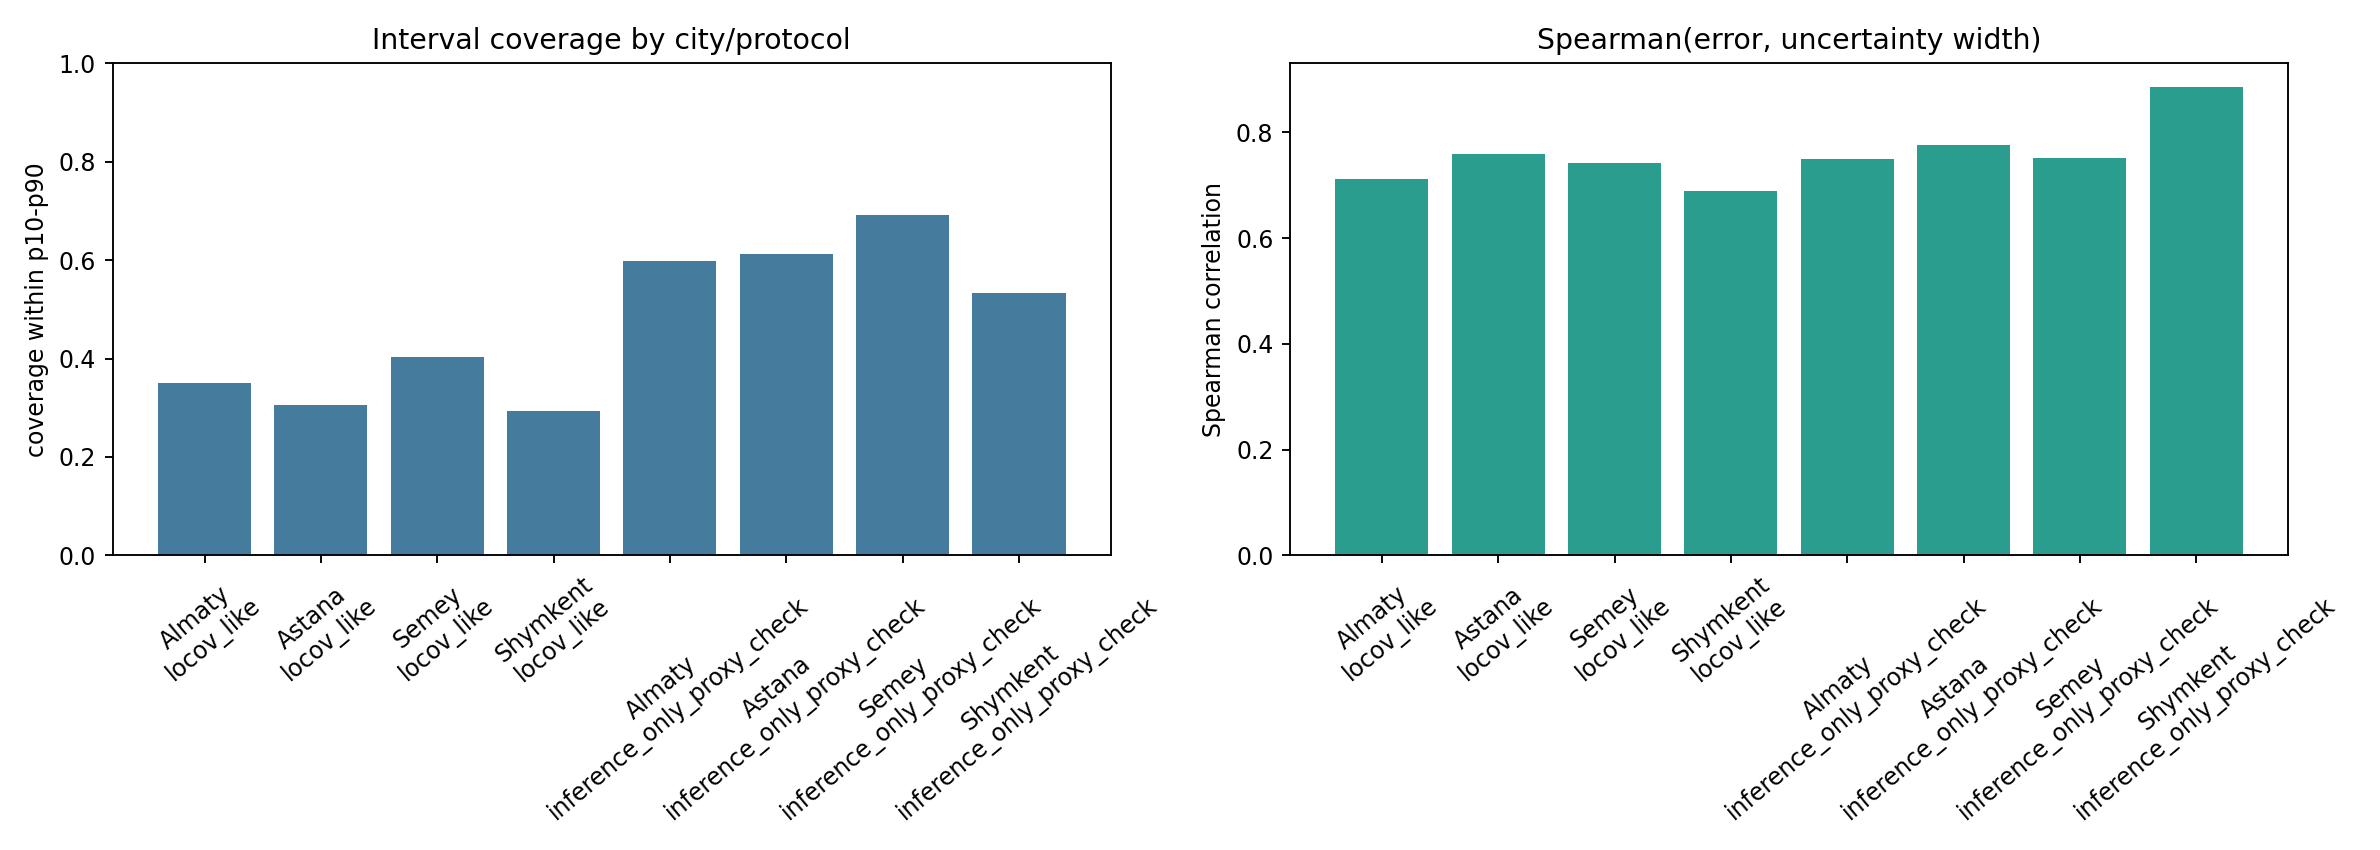
\includegraphics[width=\textwidth]{figures/fig5_uncertainty_validation_summary.png}
\caption{Summary of interval coverage and error-width alignment. Coverage is mixed across protocols, but uncertainty width carries meaningful positive alignment with proxy-target error.}
\label{fig:uncertainty-validation-unified}
\end{figure}

\subsection{Confidence bands and hotspot stability}

Where a high confidence band exists, it shows lower relative uncertainty than the low band. Almaty provides the clearest separation, from 0.044 in the high band to 0.396 in the low band. Semey also shows strong separation, from 0.061 to 0.593, despite its more mixed overall screening position.

This is the cleanest confidence-band argument in the paper. It shows that the banding scheme is not decorative: it actually sorts cells by support level in a way that can be used for screening and prioritization.

\input{tables_tex/table11_confidence_band_summary.tex}

Hotspot stability is the strongest uncertainty evidence layer. Stable classes such as \texttt{high\_value\_high\_confidence} and \texttt{medium\_value\_high\_confidence} retain much higher mean stability metrics than caution-heavy classes. This is the clearest evidence that the uncertainty-aware stage does useful screening work rather than merely adding decorative interval columns.

That makes hotspot stability the main Stage 2 takeaway. If a reviewer asks what the uncertainty layer actually adds, the answer is not "more numbers"; it is that the layer distinguishes stable screening candidates from review-heavy ones in a way that is internally coherent across the ensemble.

\begin{table}[H]
\centering
\small
\caption{Hotspot stability summary by class. Stable classes retain substantially higher mean stability metrics than caution-heavy classes across the four-city inference package.}
\label{tab:hotspot-stability-unified}
\begin{tabular}{lp{2.8cm}rrrr}
\toprule
City & Hotspot class & Cells & Mean stability & Median rel.\ unc. & Mean confidence \\
\midrule
Almaty   & high/high      & 212  & 0.777 & 0.044 & 0.738 \\
Almaty   & medium/high    & 310  & 0.784 & 0.037 & 0.745 \\
Almaty   & low/high-unc.  & 320  & 0.263 & 0.398 & 0.391 \\
Astana   & high/low       & 4    & 0.219 & 0.369 & 0.354 \\
Astana   & low/high-unc.  & 708  & 0.176 & 0.423 & 0.328 \\
Semey    & high/high      & 4    & 0.834 & 0.076 & 0.711 \\
Semey    & medium/high    & 10   & 0.825 & 0.065 & 0.717 \\
Semey    & high/low       & 19   & 0.197 & 0.590 & 0.369 \\
Semey    & low/high-unc.  & 136  & 0.292 & 0.603 & 0.369 \\
Shymkent & high/low       & 89   & 0.225 & 0.272 & 0.354 \\
Shymkent & low/high-unc.  & 1167 & 0.200 & 0.317 & 0.321 \\
\bottomrule
\end{tabular}
\end{table}



\begin{figure}[H]
\centering
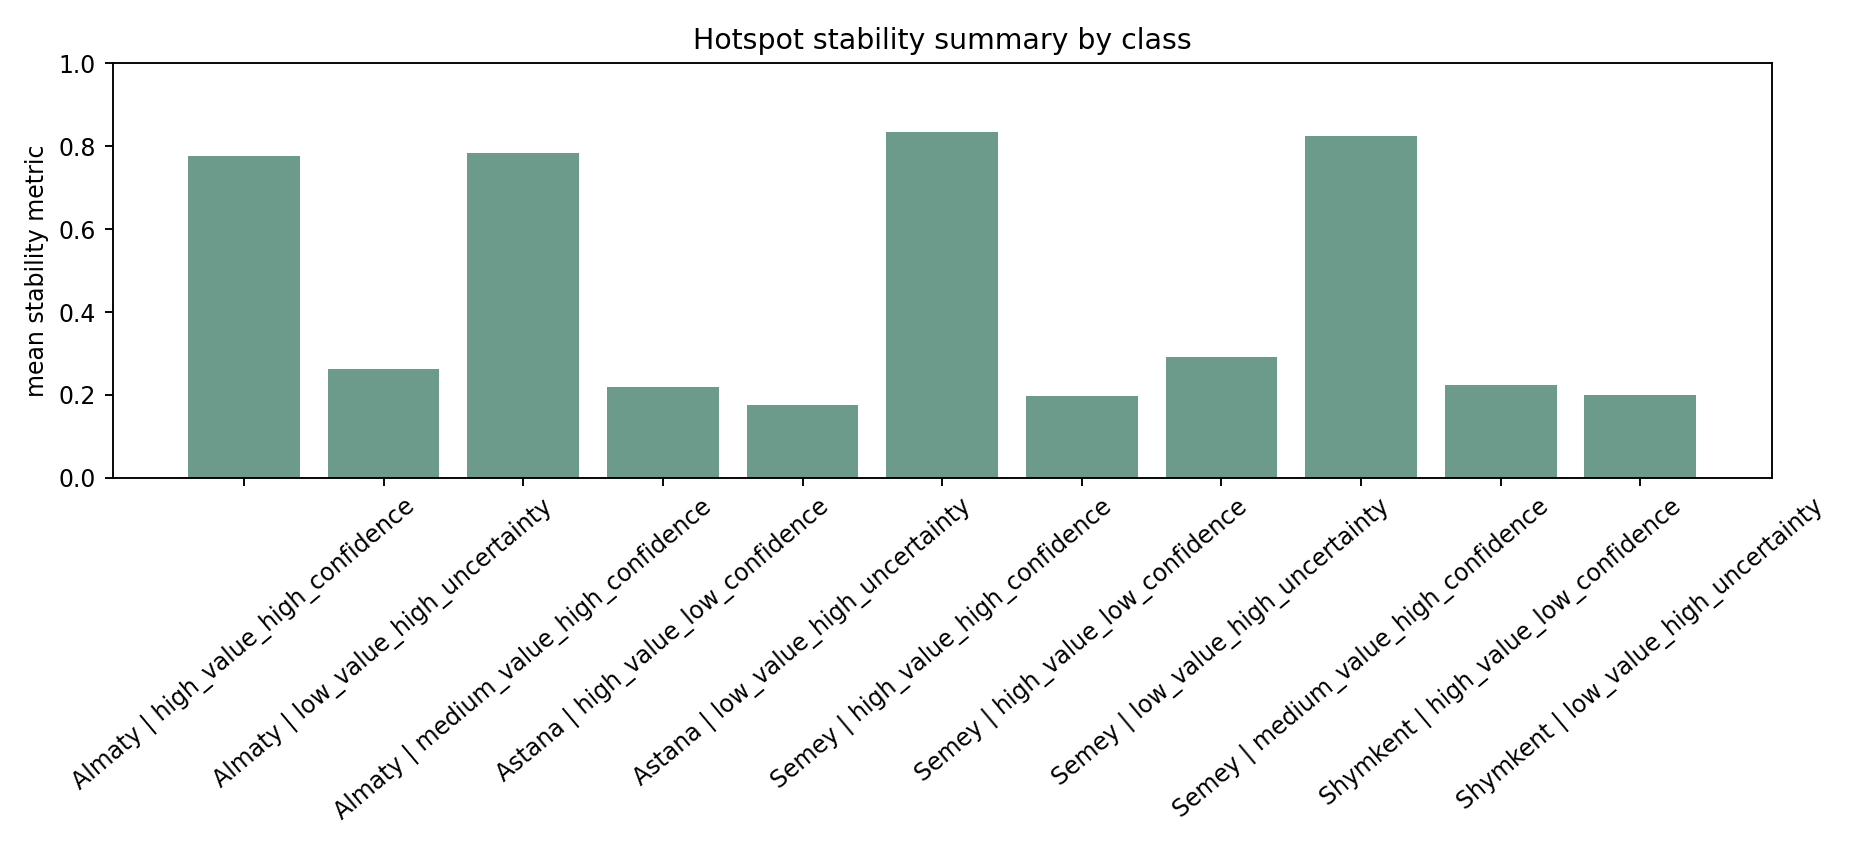
\includegraphics[width=\textwidth]{figures/fig6_hotspot_stability_summary.png}
\caption{Hotspot stability summary by class. Stable classes retain much higher mean stability than caution-heavy classes, making hotspot stability the strongest evidence layer for the uncertainty-aware stage.}
\label{fig:hotspot-stability-unified}
\end{figure}

\subsection{District and external uncertainty evidence}

The remaining uncertainty evidence layers are informative mainly as limitations. District interval coverage remains partial because true district p10/p50/p90 testing is blocked by missing district polygon/cell assignment artifacts in the light package. External disagreement alignment against WorldPop and GHS-POP is mixed or negative, so the data do not support a strong claim that uncertainty rises systematically where external disagreement increases.

These weaker layers do not invalidate Stage 2. They simply constrain it. They tell the reader that the uncertainty layer is best understood as a screening and interpretation layer, not as a full probabilistic truth model.

\begin{table}[H]
\centering
\scriptsize
\caption{District and external uncertainty evidence retained in the reference package. These layers are informative mainly as context and limitation evidence rather than as strong validation support.}
\label{tab:district-external-uncertainty-unified}
\begin{tabular}{p{2.6cm}p{2.2cm}p{1.2cm}p{3.1cm}p{5.1cm}}
\toprule
Evidence layer & Scope & Status & Available result & Limitation for interpretation \\
\midrule
District interval coverage & Almaty & partial & compared = 6; mean abs.\ error p50 = 94209.1 & True district p10/p50/p90 coverage remains blocked because frozen district polygon/cell assignments are missing. \\
District interval coverage & Astana & partial & compared = 5; mean abs.\ error p50 = 169626.3 & Treat only as partial administrative support after aggregation. \\
District interval coverage & Shymkent & partial & compared = 3; mean abs.\ error p50 = 108862.2 & Does not provide district interval validation or cell-level truth. \\
External disagreement alignment & Almaty / WorldPop & mixed & Spearman(disagreement, uncertainty) = -0.299 & External products provide structural comparison context, not ground truth. \\
External disagreement alignment & Almaty / GHS-POP & mixed & Spearman(disagreement, uncertainty) = -0.494 & Mixed or negative alignment does not support strong monotonicity claims. \\
External disagreement alignment & Astana / WorldPop & mixed & Spearman(disagreement, uncertainty) = -0.188 & Structural benchmark only. \\
External disagreement alignment & Astana / GHS-POP & mixed & Spearman(disagreement, uncertainty) = -0.251 & Structural benchmark only. \\
External disagreement alignment & Shymkent / WorldPop & mixed & Spearman(disagreement, uncertainty) = -0.422 & Structural benchmark only. \\
External disagreement alignment & Shymkent / GHS-POP & mixed & Spearman(disagreement, uncertainty) = -0.451 & Structural benchmark only. \\
\bottomrule
\end{tabular}
\end{table}



These are limitations, not fatal flaws. They narrow the claim boundary of the uncertainty-aware stage and reinforce that the correct interpretation is screening reliability rather than true uncertainty calibration.

\section{Integrated Discussion}

The main contribution of City1 is not merely a gridded map. It is a disciplined framework for producing, validating, and interpreting a calibrated proxy population surface under missing cell-level truth. This framework requires both analytical stages.

Stage 1 shows that a deterministic calibrated proxy population surface can be constructed reproducibly from open-data features, weak supervision, Random Forest learning, and official-total calibration. The baseline validation stack supports structural credibility through transfer testing, within-city robustness, district aggregation evidence, external structural comparison, ablation, and qualitative plausibility. On its own, however, this deterministic surface still risks being over-read, because a single value per cell can make stronger and weaker support conditions look equally authoritative.

Stage 2 addresses that problem directly. The uncertainty-aware extension adds calibrated ensemble intervals, confidence bands, and hotspot-screening classes so that the baseline surface is not interpreted as equally reliable everywhere. Its strongest support comes from hotspot stability and uncertainty-burden separation, with Almaty emerging as the strongest combined case. The mixed interval coverage, mixed or negative external disagreement alignment, and partial district interval evidence do not invalidate the extension, but they constrain it. They make clear that the correct output identity is reliability-aware screening rather than a true census-uncertainty model.

The two stages protect each other conceptually. Stage 1 without Stage 2 risks deterministic over-reading. Stage 2 without Stage 1 would have no stable calibrated baseline to interpret. Together, they form one coherent calibrated and uncertainty-aware proxy framework.

This dependency is the intellectual center of the paper. Stage 1 gives the framework a stable calibrated surface that can be defended as structurally plausible under missing cell-level truth. Stage 2 then prevents that surface from being read as if every cell carried the same support. The paper is strongest when both statements remain true at once.

City-specific interpretation also becomes sharper under this integrated view. Almaty is the strongest combined case because it pairs strong baseline plausibility with the clearest stable hotspot-screening support. Astana remains useful, but it is caution-heavier both in district support and in the uncertainty-aware layer. Shymkent also remains useful but caution-heavy, with weaker district support and a hotspot structure dominated by review-oriented classes. Semey sits in an intermediate position: it retains a small but meaningful stable hotspot subset while also carrying heavier relative uncertainty and a larger caution tail.

This combined interpretation changes how the framework should be used. The output is suitable for exploratory intra-urban comparison, service-planning screening, hotspot-aware triage, and cautious prioritization. It is not suitable for definitive administrative accounting below the support actually available in the evidence stack, and it should not be treated as if every cell were equally validated.

Those use cases are deliberately modest. The framework is useful when the goal is to identify relative concentration, review potentially important areas, or prioritize where more attention should go next. It is not designed to replace census operations, to automate administrative accounting, or to make unsupervised policy decisions.

The integrated framework also extends naturally into a bounded Stage 3 interpretation layer. In that layer, a tool-grounded assistant consumes the calibrated surface, the interval outputs, the confidence bands, the hotspot classes, and the explicit limitation files through controlled read-only tools rather than by generating unsupported claims from free text alone. Its role is evidence-linked explanation, reviewer-safe wording, and cautious runtime interpretation. It is not a new estimator, not a census-recovery system, and not an automated policy engine.

\section{Limitations}

\subsection{Missing cell-level census truth}

The fundamental limitation of the framework is unchanged across both stages: true cell-level census labels are unavailable. The baseline surface is therefore a calibrated proxy surface rather than a reconstruction of observed population counts per cell.

\subsection{Weak and proxy target limitation}

The deterministic stage relies on weak supervision, and much of the uncertainty-aware stage is validated against weak or proxy targets rather than observed cell-level census labels. This is a real scientific boundary and cannot be removed rhetorically. The weak target is a structured proxy allocation, not a hidden supervised truth, so some circularity is inherent to the design. The paper accepts that circularity only because it is explicit about the proxy framing and never claims to have recovered hidden census labels.

\subsection{OSM quality variation}

The feature layer depends on variable OSM quality across cities. The framework tracks completeness explicitly, but differences in open-data support still affect how strongly some results can be interpreted, especially for qualitative reading and reliability-aware screening.

\subsection{Partial district validation and district interval limits}

District comparison remains partial in both stages. In the deterministic stage, district evidence is heterogeneous across cities and should be read as partial administrative support after aggregation. In the uncertainty-aware stage, true district interval coverage remains blocked in the light package because district polygon/cell assignment artifacts are unavailable.

\subsection{External products are structural comparators, not truth}

WorldPop and GHS-POP are useful structural comparators for broad agreement and hotspot-sensitive agreement, but they are not treated as cell-level ground truth. Mixed or negative external disagreement alignment in the uncertainty-aware stage therefore constrains claims without converting the comparison into a failure against truth.

\subsection{Confidence score is not probability}

\texttt{confidence\_score} is an interpretation-confidence score, not a probability of correctness. Likewise, P10/P50/P90 are proxy uncertainty intervals, not true census-uncertainty intervals.

\subsection{Bounded LOCO-like uncertainty validation}

The held-out LOCO-like uncertainty evidence was produced in a bounded local configuration with 5 ensemble members and 60 trees per member rather than with the full 20-member inference package. This evidence remains useful but should not be overstated.

This limitation matters because it keeps the uncertainty claims bounded to the evaluation setup actually run. The runtime package is larger, but the held-out evidence used to support the manuscript is intentionally narrower and should be interpreted accordingly.

\subsection{No definitive administrative accounting or fully automated operational decisions}

The framework supports screening, interpretation, and exploratory prioritization. The tool-grounded layer can help explain frozen artifacts, but it does not support definitive fine-scale administrative accounting and should not be used as a fully automated decision system.

\subsection{No claim of true census reconstruction or true census uncertainty}

The central claim boundary of the paper is therefore deliberate. City1 does not reconstruct true cell-level census counts and does not estimate true census uncertainty. It provides an officially calibrated proxy surface together with a reliability-aware interpretation layer under missing cell-level truth.

\section*{Data and Code Availability}

The City1 framework codebase is available in the public repository \url{https://github.com/Messer490/city1-kazakhstan-proxy-population}.

Two manuscript-oriented packages are retained separately:
\begin{itemize}\setlength{\itemsep}{0pt}\setlength{\topsep}{0pt}
\item manuscript/evidence package: \pathcode{manuscript_package_city1_unified/}
\item deterministic baseline package: \pathcode{manuscript_package_v2/}
\end{itemize}

The deterministic source package records commit \pathcode{92cc78d7880af1388fcbf3a5d7aa8db57c5c4512} in its data-and-code note.

The uncertainty-aware reference run is \pathcode{city1_v3_rf500m_e20_20260618T040646Z}. Its paper-facing evidence package is retained under \pathcode{reports/paper_v3_uncertainty/city1_v3_rf500m_e20_20260618T040646Z/}. The corresponding model artifacts are stored under \pathcode{models/v3_uncertainty/city1_v3_rf500m_e20_20260618T040646Z/}, and the city outputs are stored under \pathcode{outputs/v3_uncertainty/city1_v3_rf500m_e20_20260618T040646Z/}. The uncertainty paper-facing package records commit \pathcode{389a27d} in its freeze manifest.

The tool-grounded interpretation layer is documented under \pathcode{manuscript_package_v4/}. Its evaluation artifacts are retained under \pathcode{reports/v4_llm_evaluation/}, and the runnable interface entry point is \pathcode{app_v4.py}. This layer consumes frozen artifacts and does not modify the calibrated or uncertainty-aware population outputs.

For runtime and inference use, a separate runnable snapshot is archived as \pathcode{city1_runtime_package_20260622_061747.zip}. This runtime archive is distinct from the manuscript/evidence packages and is intended for execution-oriented reuse rather than manuscript provenance.

Key external inputs are retained separately and remain subject to their original access conditions:
\begin{itemize}\setlength{\itemsep}{0pt}\setlength{\topsep}{0pt}
\item official-total reference table: \pathcode{data/external/city_population_reference_v2.csv}
\item city-status registry: \pathcode{data/external/city_status_registry_v2.csv}
\item district benchmark inputs: \pathcode{data/external/district_benchmark/}
\item Phase 5 hotspot report: \pathcode{reports/hotspot_prioritization_v3/city1_v3_rf500m_e20_20260618T040646Z/}
\item Phase 6 uncertainty-validation report: \pathcode{reports/uncertainty_validation_v3/city1_v3_rf500m_e20_20260618T040646Z/}
\end{itemize}

Third-party official and benchmark inputs remain subject to their original access conditions and licensing. An archival DOI will be added after repository deposit.

\section{Conclusion}

City1 provides a reproducible calibrated, uncertainty-aware, and tool-grounded proxy population framework for intra-urban analysis in data-scarce Kazakhstan. The framework first constructs a deterministic calibrated proxy population surface from open data, weak supervision, Random Forest modeling, and official-total calibration. It then extends that surface with calibrated ensemble intervals, confidence bands, and hotspot-prioritization classes so that the output can be interpreted in a reliability-aware way rather than as uniformly trustworthy everywhere. A bounded Stage 3 layer then exposes those frozen artifacts through controlled tools, deterministic fallback generation, optional provider generation, cache support, and reviewer-safe guardrails without altering the underlying estimates.

The central contribution is not a claim of exact cell-level reconstruction. It is a disciplined way to build a bounded proxy surface, validate it across multiple evidence layers, and then interpret its reliability in a way that prevents deterministic over-reading.

The deterministic stage shows that a calibrated proxy surface can be built and supported as structurally plausible under missing cell-level truth. The uncertainty-aware stage shows that not all parts of that surface deserve equal confidence and that hotspot stability and confidence-band separation provide the strongest screening evidence. At the same time, the framework preserves its limits honestly: interval coverage is mixed, district interval evidence remains partial, external disagreement alignment is mixed or negative, and neither stage converts the system into a true census or true uncertainty model.

Together, the two stages form one coherent framework. Stage 1 supplies the calibrated baseline; Stage 2 tells the reader how to read that baseline cautiously and where screening use is strongest. That combination is what makes City1 useful for exploratory planning, hotspot triage, and careful prioritization in data-scarce urban settings.

The final contribution is therefore intentionally bounded but mature. City1 is not a true census reconstruction model, not a true census-uncertainty model, and not an automated policy engine. It is a transparent, reproducible, officially calibrated, uncertainty-aware, and tool-grounded proxy framework for screening and interpretation under missing cell-level truth.


\bibliographystyle{plain}
\bibliography{references}

\end{document}
